\documentclass[12pt,a4paper]{article}
\usepackage[utf8]{inputenc}
\usepackage[utf8]{vietnam}
\usepackage{amsmath,amsfonts,amssymb}
\usepackage{xfrac}
\usepackage{type1cm}
\usepackage{graphicx}
%\usepackage{subfigure}
\usepackage{subfig}
\graphicspath{ {images/} }
\usepackage{multirow}
\usepackage{multicol}
\usepackage{array}
\usepackage{comment}
\usepackage{enumerate}
\usepackage[unicode]{hyperref}
\usepackage{indentfirst}
\usepackage{tikz}
\usepackage{color}
\usepackage[left=1.5cm,right=1.5cm,top=2cm,bottom=2cm]{geometry}
\usepackage[american,cuteinductors,smartlabels]{circuitikz}
\usetikzlibrary{arrows}
\usepackage{tikz}
\usetikzlibrary{calc,patterns,angles,quotes}
\usetikzlibrary{arrows, decorations.markings, calc, fadings, decorations.pathreplacing, patterns, decorations.pathmorphing, positioning}	
%\tikzstyle{every path}=[line width=1.2pt]
\title{\textbf{Bài tập ôn thi giữa kỳ\vspace{.4cm}\\Môn học Kiểm soát hệ thống điện}}
\author{SVTH: Thi Minh Nhựt -- Email: thiminhnhut@gmail.com}
\date{Thời gian: Ngày 17 tháng 10 năm 2016}
%\date{Thời gian: \today}

\begin{document}
\pagenumbering{gobble}
\maketitle
\everymath{\displaystyle}
%%
%%
\tableofcontents
%\listoffigures
%\listoftables
%\addcontentsline{toc}{section}{Tài liệu tham khảo}
\section*{Tài liệu tham khảo}
\begin{enumerate}[{[1].}]
	\item Nguyễn Hoàng Việt, \href{https://github.com/h3int2um/hethongdien/blob/master/tailieu-hethongdien/NguyenHoangViet_BaoVeRelay_TuDongHoa_HeThongDien_NXB_DHQGHCM_N2005_TBL2_492T.pdf}{\emph{Bảo vệ rơle và Tự động hóa trong hệ thống điện}}, Tái bản lần thứ hai, NXB ĐHQG TP. Hồ Chí Minh, Năm 2005.
		
	\item Nguyễn Hoàng Việt, \href{https://github.com/h3int2um/hethongdien/blob/master/tailieu-hethongdien/NguyenHoangViet_CacBaiToan_TinhNganMach_BaoVeRelay_HeThongDien_NXB_DHQGHCM_N2010_TBL3_400T.pdf}{\emph{Các bài toán tính ngắn mạch và bảo vệ rơle trong hệ thống điện}}, Tái bản lần thứ ba, NXB ĐHQG TP. Hồ Chí Minh, Năm 2010.
	
	\item Trần Quang Khánh, \href{https://github.com/h3int2um/hethongdien/blob/master/tailieu-hethongdien/TranQuangKhanh_BaoVeRelay_TuDongHoa_HeThongDien_NXB_GD_N2005_329T.pdf}{\emph{Bảo vệ rơle và Tự động hóa hệ thống điện}}, NXB Giáo dục, Năm 2005.	
\end{enumerate}
\newpage
\pagenumbering{arabic}

\newcommand{\unit}[1]{~#1} % Sau số có cách khoảng đơn vị
\newcommand{\unitp}[1]{~\left({#1}\right)} %Cặp dấu ngoặc của đơn vị
\newcommand{\pfm}[1]{\left({#1}\right)} %Cặp dấu ngoặc trong công thức
\newcommand{\chiso}[2]{\text{\textit{#1}}_{#2}}
\newcommand{\viet}[2]{#1_{\text{\textit{#2}}}}
\renewcommand{\arraystretch}{1.3}
\newpage
\section{Các vấn đề chung của bảo vệ}
\subsection{Nhiệm vụ của bảo vệ}
	\begin{itemize}
		\item Duy trì hoạt động bình thường của hệ thống và các hộ tiêu thụ trong trường hợp có sự cố.
		
		\item Phát hiện kịp thời sự cố.
		
		\item Nhanh chống tác động cắt các phần tử sự cố ra khỏi hệ thống để hạn chế hư hỏng và giảm thiệt hại.
		
		\item Tác động đến các cơ cấu khác: tự đóng lặp lại, tự đóng nguồn dự phòng,\ldots
		
		\item Hệ thống bảo vệ là phần không thể thiếu trong các mạng điện hiện đại.
		
		\item Hệ thống bảo vệ gồm tổ hợp của các phần tử cơ bản là relay.
	\end{itemize}
	
\subsection{Các yêu cầu cơ bản của hệ thống bảo vệ}
\subsubsection{Yêu cầu với bảo vệ chống ngắn mạch}
	\begin{itemize}
		\item \emph{Tính chọn lọc:} chỉ cắt phần tử hư hỏng khi ngắn mạch.
		
		\item \emph{Tác động nhanh:} bảo vệ cần tác động nhanh nhằm mục đích:
			\begin{itemize}
				\item Đảm bảo ổn định làm việc song song của các máy phát, giảm ảnh hưởng của điện áp thấp lên phụ tải.
				
				\item Giảm tác hại dòng ngắn mạch với thiết bị.
				
				\item Giảm xác suất dẫn đến hư hỏng nặng hơn.
				
				\item Nâng cao hiệu quả của thiết bị tự đóng lại.
			\end{itemize}
			
			Thời gian cắt hư hỏng: $t = t_{bv} + t_{MC}$.
			
			Việc chọn các thiết bị vừa có tính chọn lọc vừa tác động nhanh rất khó, nên người ta thực hiện phương pháp là \emph{cắt nhanh không chọn lọc}, sau đó dùng các \emph{thiết bị tự đóng} lại để đóng các phần tử bị cắt không chọn lọc.
			
		\item \emph{Độ nhạy:} mỗi bảo vệ cần tác động khi có sự cố trong vùng bảo vệ của mình với bảo vệ chính và bảo vệ dự trữ.
		
		\item \emph{Độ tin cậy:} bảo vệ phải chắc chắn tác động khi ngắn mạch xảy ra trong vùng được giao bảo vệ và không tác động đối với các chế độ mà nó không có nhiệm vụ tác động.
		
		Để bảo vệ tác động tin cậy: dùng sơ đồ đơn giản, giảm số lượng relay và tiếp xúc, cấu tạo đơn giản, chế độ và lắp ráp đảm bảo chất lượng, kiểm tra thường xuyên trong quá trình vận hành.
		
		\item \emph{Tính kinh tế:} các relay cần đảm bảo yêu cầu kỹ thuật và tính kinh tế.
	\end{itemize}

\subsubsection{Yêu cầu với bảo vệ chống các chế độ làm việc không bình thường}
	Cần tác động chọn lọc, độ nhạy và tin cậy, không đề cập đến tác động nhanh.
	
\subsection{Các bộ phận của hệ thống bảo vệ}
	Hệ thống bảo vệ gồm 2 thành phần chính là: \emph{phần đo lường} và \emph{phần logic}.
	
	\begin{itemize}
		\item \emph{Phần đo lường:} ghi nhận thông tin tình trạng của phần tử được bảo vệ, ghi nhận sự cố xuất hiện và tình trạng làm việc không bình thường và gửi tín hiệu đến phần logic. Ghi nhận thông tin của phần tử được bảo vệ qua các bộ biến đổi đo lường sơ cấp \emph{biến dòng -- $BI$} và \emph{biến áp -- $BU$}.
			\begin{itemize}
				\item Đo lường sơ cấp: biến áp và biến dòng.
				
				\item Đo lường thứ cấp và các bộ phận so sánh.
			\end{itemize}
		
		\item \emph{Phần logic tiếp nhận tín hiệu từ phần đo lường:} Nếu giá trị, thứ tự và tổng hợp các tín hiệu phù hợp với chương trình định trước nó sẽ phát tín hiệu điều khiển (cắt máy cắt hoặc báo hiệu qua thiết bị điều khiển).
			\begin{itemize}
				\item Phần logic của bảo vệ.
				
				\item Mạch thực hiện điều khiển máy cắt.
			\end{itemize}
			
		\item Ngoài ra, cần có \emph{nguồn thao tác:} nguồn một chiều và nguồn xoay chiều.
	\end{itemize}
	
\subsection{Các nguyên lý cơ bản của bảo vệ relay}
	\begin{itemize}
		\item \emph{Bảo vệ dòng cực đại:} dòng điện khởi động của bảo vệ lớn hơn dòng làm việc cực đại chạy qua đối tượng được bảo vệ.
		
		\item \emph{Bảo vệ cắt nhanh:} dòng điện làm việc của bảo vệ lớn hơn dòng ngắn mạch cực đại tại điểm sau đối tượng được bảo vệ.

		\item \emph{Bảo vệ kết hợp quá dòng và sụt áp:} bảo vệ thực hiện theo nguyên lý $AND$.
		
		\item \emph{Bảo vệ bằng bộ lọc:} bảo vệ được chỉnh định theo thành phần thứ tự nghịch hoặc thứ tự không của dòng điện và điện áp.
		
		\item \emph{Bảo vệ theo hướng dòng công suất:} bảo vệ được thực hiện với sự tham gia của relay công suất, xác định hướng của dòng điện ngắn mạch.
		
		\item \emph{Bảo vệ khoảng cách:} bảo vệ thực hiện theo phương pháp đo điện trở từ điểm đặt bảo vệ đến điểm ngắn mạch.
		
		\item \emph{Bảo vệ so lệch dòng điện:} dựa trên so sánh trị số và góc pha của dòng điện ở đầu và cuối vùng bảo vệ.
		
		\item \emph{Bảo vệ so lệch pha của dòng điện:} dựa vào so sánh pha của dòng điện ở hai đầu đường dây được bảo vệ.
		
	\end{itemize}

\newpage
\section{Bảo vệ quá dòng điện}
\subsection{Nguyên tắc bảo vệ}
	\subparagraph{Nguyên tắc} Bảo vệ tác động khi \emph{dòng điện qua chỗ đặt thiết bị bảo vệ tăng quá giá trị đặt trước}.	

	\subparagraph{Chức năng} Bảo vệ chống các hiện tượng ngắn mạch.
	
	\subparagraph{Phân loại} Có thể chia bảo vệ dòng điện thành: \emph{bảo vệ dòng điện cực đại} \emph{bảo vệ dòng điện cắt nhanh}.
		\begin{itemize}
			\item Hai loại bảo vệ trên khác nhau về: \emph{yêu cầu tác động chọn lọc} và \emph{vùng bảo vệ tác động}.
			
			\item \emph{Bảo vệ dòng điện cực đại:}
				\begin{itemize}
					\item Nguyên lý: bảo vệ quá dòng có thời gian trì hoãn.
					
					\item Vùng bảo vệ: gồm phần tử bảo vệ và các phần tử lân cận.
				\end{itemize}
				
			\item \emph{Bảo vệ dòng điện cắt nhanh:}
				\begin{itemize}
					\item Nguyên lý: bảo vệ quá dòng tác động tức thời chỉnh định theo dòng ngắn mạch bên ngoài.
					
					\item Vùng bảo vệ: chỉ một phần của phần tử được bảo vệ.
				\end{itemize}
		\end{itemize}
		
	\subparagraph{Mã số relay}
		\begin{itemize}
			\item Bảo vệ dòng điện cực đại: $51$.
			\item Bảo vệ dòng điện cắt nhanh: $50$.
		\end{itemize}
		
\subsection{Bảo vệ dòng điện cực đại}
	\begin{itemize}
		\item \emph{Nguyên tắc đặt thời gian trì hoãn:} đặt theo nguyên tắc từng cấp, thời gian tăng dần tính từ hộ tiêu thụ cho đến nguồn.
		
		\item \emph{Dòng khởi động của bảo vệ:} $\viet{I}{kđ} > I_{lvmax}$.
		
		\item Công thức tính toán dòng khởi động bảo vệ:
			\begin{itemize}
				\item Dòng khởi động của bảo vệ: $\viet{I}{kđ} = \dfrac{K_{at} K_{mm}}{K_{tv}} \times I_{lvmax}$.
				
				\item Dòng khởi động relay: $\viet{I}{kđR} = \dfrac{K_{at} K_{mm}}{K_{tv} n_{BI}} \times I_{lvmax} = \dfrac{\viet{I}{kđ}}{n_{BI}}$.
				
				\item[$\ast$] Trong đó: $K_{at}$ là hệ số an toàn, $K_{mm}$ là hệ số mở máy động cơ (thường cho $K_{mm} = 2 \div 3$), $K_{tv}$ là hệ số trở về, $n_{BI}$ là tỉ số biến dòng, $I_{lvmax}$ là dòng làm việc cực đại.
			\end{itemize}
				
		\item Công thức tính toán độ nhạy của bảo vệ:
			\begin{itemize}
				\item Độ nhạy bảo vệ chính: $K_{nhbvc} = \dfrac{I_{Nmin}}{\viet{I}{kđ}}$, với $I_{Nmin}$ là dòng ngắn mạch nhỏ nhất của phần tử bảo vệ chính. Yêu cầu: $K_{nhbvc} > 1.5$.
				
				\item Độ nhạy bảo vệ dự trữ: $K_{nhbvdtr} = \dfrac{I_{Nmin}}{\viet{I}{kđ}}$, với $I_{Nmin}$ là dòng ngắn mạch nhỏ nhất của các phần tử bảo vệ lân cận. Yêu cầu: $K_{nhbdtr} > 1.2$.
			\end{itemize}
			
		\item Dòng khởi động của bảo vệ phụ thuộc vào $K_{tv}$ và $I_{lvmax}$: muốn giảm dòng khởi động để tăng độ nhạy cho bảo vệ cần chọn relay có hệ số trở về cao.
		
		\item Thời gian tác động của bảo vệ:
			\begin{itemize}
				\item \emph{Relay dòng điện có đặc tính thời gian độc lập:}
					\begin{list}{+}{}
						\item Thời gian trì hoãn tạo ra nhờ vào \emph{relay thời gian} và \emph{không phụ thuộc vào dòng ngắn mạch}.
						
						\item Thời gian tác động: $t_2 = \max{t_i} + \Delta t$. Thường chọn $\Delta t = 0.35 \div 0.6 \unit{s}$. Chọn thời gian $t_i$ lớn nhất để tính thời gian tác động cho bảo vệ.
						
					\end{list}
					
				\item \emph{Relay dòng điện có đặc tính thời gian phụ thuộc:}
					\begin{list}{+}{}
						\item Relay làm việc với thời gian xác định nào đó khi \emph{dòng điện vượt quá giá trị khởi động}. Thời gian tác động của relay \emph{phụ thuộc vào dòng điện qua relay}, thời gian làm việc giảm khi dòng tăng cao.
						
						\item Phương trình đường cong của Mỹ:
							\begin{itemize}
								\item Đường cong có độ dốc $U_1$:
									\begin{align*}
										\viet{t}{tđ} = \pfm{0.0226 + \dfrac{0.01014}{m^{0.02} - 1}}TD; \qquad t_{tv} = \dfrac{1.08TD}{1-m^2}
									\end{align*}
									
								\item Đường cong có độ dốc $U_2$:
									\begin{align*}
										\viet{t}{tđ} = \pfm{0.18 + \dfrac{5.95}{m^{2} - 1}}TD; \qquad t_{tv} = \dfrac{5.95TD}{1-m^2}
									\end{align*}
									
								\item Đường cong có độ dốc $U_3$:
									\begin{align*}
										\viet{t}{tđ} = \pfm{0.0963 + \dfrac{3.88}{m^{2} - 1}}TD; \qquad t_{tv} = \dfrac{3.88TD}{1-m^2}
									\end{align*}
									
								\item Đường cong có độ dốc $U_4$:
									\begin{align*}
										\viet{t}{tđ} = \pfm{0.0352 + \dfrac{5.67}{m^{2} - 1}}TD; \qquad t_{tv} = \dfrac{5.67TD}{1-m^2}
									\end{align*}
									
								\item Trong đó:
									\begin{list}{}{}
										\item $\viet{t}{tđ}$: thời gian tác động của bảo vệ quá dòng $(s)$.
										\item $t_{tv}$: thời gian trở về của bảo vệ $(s)$.
										\item $TD$: hệ số chọn thời gian (trị đặt thời gian).
										\item $m = \dfrac{I_{NM}}{\viet{I}{đặt}}$: bộ số dòng ngắn mạch so với dòng đặt của bảo vệ.
										
										Với $\viet{I}{đặt} = \viet{I}{kđ} = I_s = I_p = I$ (các ký hiệu dòng đặt được dùng).
									\end{list}
							\end{itemize}
							
						\item Phương trình đường cong theo tiêu chuẩn IEC:
							\begin{itemize}
								\item Đường cong dốc chuẩn $SIT-C1$:
									\begin{align*}
										\viet{t}{tđ} = \dfrac{0.14TMS}{m^{0.02} - 1} = \dfrac{0.14T}{2.97\pfm{m^{0.02} - 1}}; \qquad t_{tv} = - \dfrac{1.08TMS}{m^2 - 1}; \qquad TMS = \dfrac{T}{2.97}
									\end{align*}

								\item Đường cong rất dốc $VIT-C2$:
									\begin{align*}
										\viet{t}{tđ} = \dfrac{13.5TMS}{m - 1} = \dfrac{13.5T}{1.5\pfm{m - 1}}; \qquad t_{tv} = - \dfrac{13.5TMS}{m - 1}; \qquad TMS = \dfrac{T}{1.5}
									\end{align*}

								\item Đường cong cực dốc $EIT-C3$:
									\begin{align*}
										\viet{t}{tđ} = \dfrac{80TMS}{m^2 - 1} = \dfrac{80T}{0.808\pfm{m^2 - 1}}; \qquad t_{tv} = - \dfrac{80TMS}{m^2 - 1}; \qquad TMS = \dfrac{T}{0.808}
									\end{align*}

								\item Đường cong siêu dốc $UIT$:
									\begin{align*}
										\viet{t}{tđ} = \dfrac{315TMS}{m^{2.5} - 1} = \dfrac{315T}{2.97\pfm{m^{2.5} - 1}}; \qquad TMS = \dfrac{T}{2.97}
									\end{align*}

								\item Đường cong dành cho chống chạm đất $RI$:
									\begin{align*}
										\viet{t}{tđ} = \dfrac{0.315T}{0.399 - \dfrac{0.236}{m}}
									\end{align*}

								\item Đường cong có thời gian tác động lâu $C4$:
									\begin{align*}
										\viet{t}{tđ} = \dfrac{120TMS}{m-1}; \qquad t_{tv} = \dfrac{120TMS}{m-1}
									\end{align*}

								\item Trong đó: 
									\begin{list}{}{}
										\item $TMS$: hệ số chọn thời gian, giá trị đặt thời gian, hệ số nhân thời gian (giống hệ số $TD$ của Mỹ, ký hiệu khác là $T_p, K$).
										\item $T$: thời gian tác động của bảo vệ lúc ngắn mạch bằng $10$ lần giá trị đặt dòng điện $\pfm{m=10}$ với $m = \dfrac{I_{NM}}{\viet{I}{đặt}}$.
									\end{list}

								\item Nhận xét $\viet{t}{tđ} = k_1 TMS = k_1 TD = k_2 T$ với $k_1, k_2$ là các hằng số.
							\end{itemize}
					\end{list}
			\end{itemize}
	\end{itemize}

\subsection{Bảo vệ dòng điện cắt nhanh}
	\begin{itemize}
		\item Bảo vệ dòng cắt nhanh: là bảo vệ chống quá dòng tác động một cách tức thời.
		
		\item \emph{Nguyên lý:} bảo vệ dòng cắt nhanh đảm bảo tính chọn lọc dựa vào chọn dòng điện khởi động lớn hơn dòng điện ngắn mạch lớn nhất qua chỗ đặt bảo vệ khi ngắn mạch ở ngoài phần tử được bảo vệ (cuối vùng bảo của phần tử được bảo vệ).
		
		\item Dòng khởi động bảo vệ: $\viet{I}{kđ} > I_{Nmax}$.
		
		\item Các công thức tính toán dòng khởi động bảo vệ:
			\begin{itemize}
				\item Dòng khởi động của bảo vệ: $\viet{I}{kđ} = K_{at}I_{Nmax}$.
				
				\item Dòng khởi động relay: $\viet{I}{kđ} = \dfrac{K_{at}I_{Nmax}}{n_{BI}} = \dfrac{\viet{I}{kđ}}{n_{BI}}$.
				
				\item[$\ast$] Trong đó: $K_{at}$ là hệ số an toàn, $n_{BI}$ là tỉ số biến dòng, $I_{Nmax}$ là dòng ngắn mạch lớn nhất ngoài vùng bảo vệ.	
			\end{itemize}

		\item Độ nhạy của bảo vệ: $K_{nh} = \dfrac{I_{Nmin}}{\viet{I}{kđ}}$, với $I_{Nmin}$ là dòng ngắn mạch nhỏ nhất trong vùng bảo vệ cắt nhanh.		
	\end{itemize}
	
\subsection{Bảo vệ dòng điện cực đại có kiểm tra áp}
	\begin{itemize}
		\item Dòng khởi động của bảo vệ dòng điện cực đại có giá trị lớn và đôi khi không đảm bảo yêu cầu về độ nhạy.
		
		\item Để tăng cường bảo vệ, người ta dùng relay điện áp làm bộ phận khởi động.
		
		\item Cấu trúc của bảo vệ dòng điện cực đại có kiểm tra áp: hình \ref{Fig:sodocautruc-bvdongdien-kiemtraap}.
			\begin{figure}[!h]
				\begin{center}					
					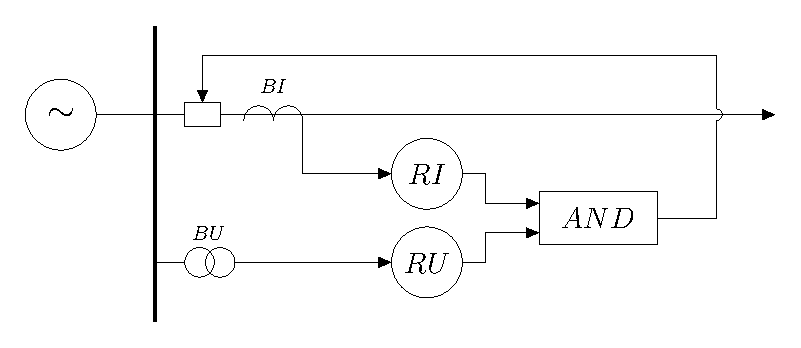
\includegraphics[scale=1]{diagram-draw-tikz/Figure-cautruc-baove-dongdiencokiemtraap.pdf} 
				\end{center}
				\caption{Sơ đồ cấu trúc của bảo vệ dòng điện có kiểm tra áp} \label{Fig:sodocautruc-bvdongdien-kiemtraap}
			\end{figure}

			\item Mã số relay: $51V$.
		
		\item Bảo vệ chỉ tác động khi relay giảm áp $RU$ đã tác động. Giá trị đặt cho relay giảm áp $RU$ sao cho nó tác động khi có ngắn mạch (vì khi ngắn mạch điện áp giảm rất nhiều).
		
		\item Dòng khởi động của $RI$:
			\begin{itemize}
				\item Dòng khởi động bảo vệ: $\viet{I}{kđ} = \dfrac{K_{at}}{K_{tv}} \times I_{lv}$
				
				\item Dòng khởi động relay: $\viet{I}{kđR} = \dfrac{K_{at}}{K_{tv}n_{BI}} \times I_{lv} = \dfrac{\viet{I}{kđ}}{n_{BI}}$
				
				\item[$\ast$] Trong đó: $K_{at}$ là hệ số an toàn, $K_{tv}$ là hệ số trở về, $n_{BI}$ là tỉ số biến dòng, $I_{lv}$ là dòng làm việc (thường chọn $I_{lv} \leq \dfrac{I_{lvmax}}{1.5}$, với $I_{lvmax}$ là dòng làm việc cực đại).
			\end{itemize}
		
		\item Độ nhạy của bảo vệ $RI$: $K_{nh} = \dfrac{I_{Nmin}}{\viet{I}{kđ}}$, với $I_{Nmin}$ là dòng ngắn mạch nhỏ nhất trong vùng bảo.
		
		\item Điện áp khởi động của relay giảm áp $RU$ được chọn theo yêu cầu:
			\begin{itemize}
				\item Relay giảm áp $RU$ không được tác động đối với điện áp làm việc tối thiểu.
				
				\item Relay giảm áp $RU$ phải trở về trạng thái bình thường sau khi sự cố ngắn mạch được loại trừ.
			\end{itemize}
			
		\item Chọn điện áp khởi động cho relay giảm áp $RU$: $\viet{U}{kđ} = \pfm{0.7 \div 0.75}U_{lvmax}$.
		
		\item Độ nhạy của bảo vệ $RU$: $K_{nh} = \dfrac{\viet{U}{kđ}}{U_{Nmax}} \geq 1.5$, với $U_{Nmax}$ là điện áp lớn nhất khi ngắn mạch ở cuối vùng bảo vệ.
	\end{itemize}
	
\subsection{Bảo vệ dòng điện ba cấp}
	\begin{itemize}
		\item Bảo vệ dòng điện ba cấp gồm các bảo vệ: \emph{cấp $I$ -- bảo vệ cắt nhanh tức thời}, \emph{cấp $II$ -- bảo vệ cắt nhanh có thời gian}, \emph{cấp $III$ -- bảo vệ dòng điện cực đại}.				
		\item Mạng điện minh họa bảo vệ dòng điện ba cấp: hình \ref{Fig:bvdongdien-bacap}.
			\begin{figure}[!h]
				\begin{center}					
					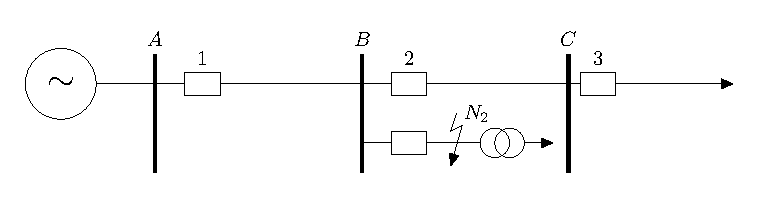
\includegraphics[scale=1]{diagram-draw-tikz/Figure-baove-dongdienbacap.pdf} 
				\end{center}
				\caption{Sơ đồ cấu trúc của bảo vệ dòng điện ba cấp} \label{Fig:bvdongdien-bacap}
			\end{figure}
			
			\begin{itemize}
				\item Vùng bảo vệ cấp $I$ của đoạn gồm $A$ và $B$ với dòng khởi động bảo vệ: $\viet{I}{kđA}^{I} = K_{at}I_{NBmax}$ với $N_{NBmax}$ là dòng ngắn mạch lớn nhất ở thanh cái $B$.
				
				\item Vùng bảo vệ cấp $II$ là đoạn gồm $A$ và $B$ và một phần đoạn kế nối vào trạm $B$, cấp $II$ là bảo vệ dự trữ cho cấp $I$:
					\begin{list}{+}{}
						\item Thời gian của bảo vệ cấp $II$: $t_{A}^{II} = t_{A}^{I} + \Delta t$.
						
						\item Dòng khởi động cấp $II$: $\viet{I}{kđA}^{II} = K_{at}\viet{I}{kđB}^{I} = K_{at}I_{N2max}$.
					\end{list}
					
				\item Vùng bảo vệ cấp $III$: thời gian tác động $t_{A}^{III} = t_{A}^{II} + \Delta t$.
			\end{itemize}
	\end{itemize}

\subsection{Đánh giá bảo vệ quá dòng điện}
	\begin{itemize}
		\item \emph{Ưu điểm bảo vệ dòng điện cực đại:} đơn giản, độ tin cậy cao. Bảo vệ tác động chọn lọc trong mạng hình tia với một nguồn cung cấp.
		
		\item \emph{Nhược điểm bảo vệ dòng điện cực đại:} thời gian ngắn mạch khá lớn (nhất là các đoạn gần nguồn, trong khi đó ngắn mạch ở gần nguồn cần được cắt nhanh để đảm bảo ổn định của hệ thống), có độ nhạy kém trong mạng phân nhiều nhánh và phụ tải lớn.
		
		\item Được dùng phổ biến trong tất cả các cấp điện áp.
		
		\item \emph{Ưu điểm bảo vệ dòng điện cắt nhanh:} tác động nhanh, đơn giản, độ tin cậy cao.
		
		\item \emph{Nhược điểm bảo vệ dòng điện cắt nhanh:} vùng tác động của bảo vệ không bao gồm toàn bộ đường dây.
		
		\item \emph{Bảo vệ dòng điện ba cấp:} cần kết hợp với bảo vệ cắt nhanh và bảo vệ dòng điện cực đại.
	\end{itemize}
	
\newpage
\subsection{Bài tập Bảo vệ quá dòng điện}
	\begin{enumerate}[1.]
		\item \label{ex:bt1-bvdongdien} Cho mạng điện như hình \ref{Fig:bt1-bvdongdien}, các số liệu tính toán cho ở bảng \ref{Tab:bt1-bvdongdien-dongdien} và bảng \ref{Tab:bt1-bvdongdien-thoigian}.					

			\begin{figure}[!h]
				\vspace{-.5cm}
				\begin{center}
					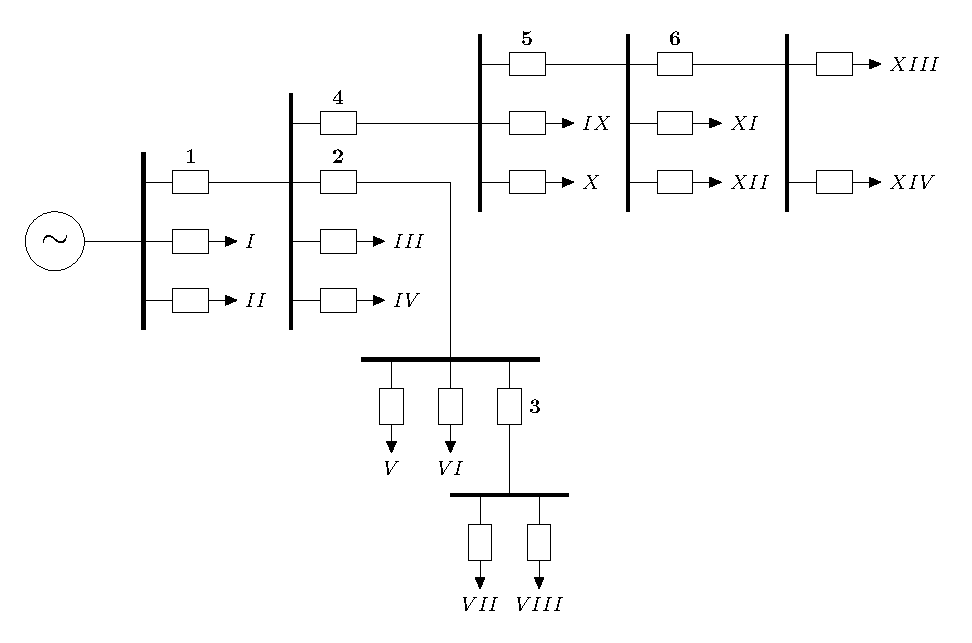
\includegraphics[scale=1]{diagram-draw-tikz/Figure-baitap-baovedongdien-bt1.pdf} 				
				\end{center}
				\vspace{-1cm}
				\caption{Sơ đồ mạng điện trong bài tập \ref{ex:bt1-bvdongdien} -- bảo vệ dòng điện với thời gian độc lập} \label{Fig:bt1-bvdongdien}
			\end{figure}		
			
			\begin{table}[!h]
				\begin{center}		
					\begin{tabular}{|c|c|c|c|c|c|c|c|} \hline 
							\multirow{2}{.7cm}{\textbf{P.A}} & \multicolumn{7}{c|}{\textbf{Dòng tải} $\mathbf{(A)}$} \\ \cline{2-8}
							 & $I_{I} + I_{II}$ & $I_{III} + I_{IV}$ & $I_{V} + I_{VI}$ & $I_{VII} + I_{VIII}$ & $I_{IX} + I_{X}$ & $I_{XI} + I_{XII}$ & $I_{XIII} + I_{XIV}$ \\ \hline
							\textbf{1} & 215 & 37 & 80 & 34 & 78 & 24 & 68 \\ \hline 
							\textbf{2} & 315 & 68 & 19 & 51 & 25 & 36 & 24 \\ \hline 
							\textbf{3} & 135 & 71 & 63 & 48 & 70 & 29 & 41 \\ \hline 
							\multicolumn{8}{|c|}{\textbf{Dòng ngắn mạch tại thanh góp có phụ tải} $\mathbf{(A)}$} \\ \hline 
							 & $I_{I} + I_{II}$ & $I_{III} + I_{IV}$ & $I_{V} + I_{VI}$ & $I_{VII} + I_{VIII}$ & $I_{IX} + I_{X}$ & $I_{XI} + I_{XII}$ & $I_{XIII} + I_{XIV}$ \\ \hline 
							\textbf{1} & 2110 & 1550 & 1100 & 770 & 1200 & 1080 & 950 \\ \hline 
							\textbf{2} & 1100 & 840 & 740 & 590 & 780 & 680 & 600 \\ \hline 
							\textbf{3} & 1430 & 1090 & 890 & 680 & 930 & 790 & 640 \\ \hline 
							\multicolumn{8}{|c|}{\textbf{Dòng ngắn mạch tại cuối đường} $\mathbf{(A)}$} \\ \hline 
							 & $I_{I} + I_{II}$ & $I_{III} + I_{IV}$ & $I_{V} + I_{VI}$ & $I_{VII} + I_{VIII}$ & $I_{IX} + I_{X}$ & $I_{XI} + I_{XII}$ & $I_{XIII} + I_{XIV}$ \\ \hline
							\textbf{1} & 1500 & 730 & 930 & 670 & 1100 & 690 & 710 \\ \hline 
							\textbf{2} & 850 & 550 & 650 & 510 & 680 & 510 & 530 \\ \hline 
							\textbf{3} & 1100 & 630 & 760 & 570 & 710 & 600 & 610 \\ \hline 
					\end{tabular}		
				\end{center}
				\caption{Dòng làm việc và dòng ngắn mạch của các phần tử trên hình \ref{Fig:bt1-bvdongdien}} \label{Tab:bt1-bvdongdien-dongdien}
			\end{table}				
			
		\begin{table}[!h]
				\begin{center}
					\begin{tabular}{|c|c|c|c|c|c|c|c|c|c|c|c|c|c|c|} \hline 
						\textbf{P.A} & $t_{I}$ & $t_{II}$ & $t_{III}$ & $t_{IV}$ & $t_{V}$ & $t_{VI}$ & $t_{VII}$ & $t_{VIII}$ & $t_{IX}$ & $t_{X}$ & $t_{XI}$ & $t_{XII}$ & $t_{XIII}$ & $t_{XIV}$ \\ \hline 
						\textbf{1} & 1 & 1 & 0.5 & 2.5 & 0.5 & 1 & 0 & 0 & 1 & 1.5 & 0.5 & 1 & 0.5 & 1.5 \\ \hline 
						\textbf{2} & 1.5 & 2 & 2 & 1.1 & 1 & 2.5 & 1 & 1.5 & 1.5 & 1.5 & 1 & 0.5 & 1 & 0.5 \\ \hline 
						\textbf{3} & 4 & 1 & 3 & 1.5 & 2 & 1 & 1 & 1.5 & 1 & 2 & 1 & 1 & 0.5 & 1 \\ \hline					
						\end{tabular}
				\end{center}
				\caption{Thời gian tại các phụ tải trên hình \ref{Fig:bt1-bvdongdien}} \label{Tab:bt1-bvdongdien-thoigian}
			\end{table}	
			
		\subparagraph{Yêu cầu}
			\begin{enumerate}[a.]
				\item Chọn thời gian tác động của bảo vệ dòng điện cực đại có đặc tính thời gian độc lập đặt tại các vị trí máy cắt $1, 2, 3, 4, 5, 6, 7$. Cho $\Delta t = 0.5\unit{s}$.
				
				\item Chọn tỉ số máy biến dòng, dòng khởi động bảo vệ (sơ đồ $BI$ nối hình sao). Kiểm tra độ nhạy, cho $K_{at} = 1.2$ và $K_{tv} = 0.85$.
			\end{enumerate}

		\subparagraph{Bài giải}
			\begin{enumerate}[\it a.]
				\item \emph{Chọn thời gian tác động của relay bảo vệ dòng cực đại có đặc tính thời gian độc lập}
					\begin{itemize}
						\item \textbf{Phương án 1}
							\begin{itemize}
								\item Relay BV $6$: $t_6 = \max\pfm{t_{XIII}, t_{XIV}} + \Delta t = \max\pfm{0.5; 1.5} + 0.5 = 1.5 + 0.5 = 2\unit{s}$.
								
								\item Relay BV $5$: $t_5 = \max\pfm{t_{XI}, t_{XII}, t_{6}} + \Delta t = \max\pfm{0.5; 1; 2} + 0.5 = 2 + 0.5 = 2.5\unit{s}$.
								
								\item Relay BV $4$: $t_4 = \max\pfm{t_{IX}, t_{X}, t_{5}} + \Delta t = \max\pfm{1; 1.5; 2.5} + 0.5 = 2.5 + 0.5 = 3\unit{s}$.
								
								\item Relay BV $3$: $t_3 = \max\pfm{t_{VII}, t_{VIII}} + \Delta t = \max\pfm{0; 0} + 0.5 = 0 + 0.5 = 0.5\unit{s}$.
								
								\item Relay BV $2$: $t_2 = \max\pfm{t_{V}, t_{VI}, t_{3}} + \Delta t = \max\pfm{0.5; 1; 0.5} + 0.5 = 1 + 0.5 = 1.5\unit{s}$.
								
								\item Relay BV $1$: $t_1 = \max\pfm{t_{III}, t_{IV}, t_{2}, t_{4}} + \Delta t = \max\pfm{0.5; 2.5; 1.5; 3} + 0.5 = 3 + 0.5 = 3.5\unit{s}$.
							\end{itemize}
							
						\item Thực hiện tương tự cho \textbf{Phương án 2} và \textbf{Phương án 3}, được kết quả trong bảng \ref{Tab:bt1-bvdongdien-thoigian-tacdong-baove}.
						
							\begin{table}[!h]
								\begin{center}
									\begin{tabular}{|c|c|c|c|c|c|c|}\hline 
									\multirow{2}{2.3cm}{\textbf{Phương án}} & \multicolumn{6}{c|}{\textbf{Thời gian tác động $\mathbf{(s)}$}} \\ \cline{2-7} 
									 & $t_1$ & $t_2$ & $t_3$ & $t_4$ & $t_5$ & $t_6$ \\\hline 
									\textbf{1} & 3.5 & 1.5 & 0.5 & 3 & 2.5 & 2 \\ \hline 
									\textbf{2} & 3.5 & 3 & 2 & 2.5 & 2 & 1.5 \\ \hline 
									\textbf{3} & 3.5 & 2.5 & 2 & 2.5 & 2 & 1.5 \\ \hline 
									\end{tabular} 
								\end{center}
								\caption{Thời gian tác động của bảo vệ dòng điện cực đại cho các phương án trong bài tập \ref{ex:bt1-bvdongdien}} \label{Tab:bt1-bvdongdien-thoigian-tacdong-baove}
							\end{table}
					\end{itemize}

				\item \emph{Chọn tỉ số máy biến dòng, tính dòng khởi động bảo vệ, dòng khởi động relay và độ nhạy bảo vệ chính, độ nhạy bảo vệ dự trữ}
					\begin{itemize}
						\item \textbf{Phương án 1}
							\begin{itemize}
								\item Relay BV $6$:
									\begin{itemize}
										\item Dòng làm việc cực đại: $I_{lvmax_{6}} = I_{t} = I_{XIII} + I_{XIV} = 68 \unit{A}$.
											\begin{list}{+}{}											
												\item Chọn tỉ số $BI$ là $75/5$ và $n_{BI_6} = 15$.
												
												\item Dòng khởi động bảo vệ: $I_{\chiso{kđbv}{6}} = \dfrac{K_{at} \times I_{lvmax_{6}}}{K_{tv}} = \dfrac{1.2 \times 68}{0.85} = 96 \unit{A}$.
												
												\item Dòng khởi động relay: $I_{\chiso{kđR}{6}} = \dfrac{I_{\chiso{kđbv}{6}}}{n_{BI_6}} = \dfrac{96}{15} = 6.4 \unit{A}$.
											\end{list}
											
										\item Độ nhạy:
										\begin{list}{+}{}
												\item Bảo vệ chính: $K_{nhbvc} = \dfrac{I_{NminTG}}{I_{\chiso{kđbv}{6}}} = \dfrac{950}{96} = 9.90$.
												
												\item Bảo vệ dự trữ: $K_{nhbvdtr} = \dfrac{I_{Nmin\text{\textit{ĐD}}}}{I_{\chiso{kđbv}{6}}} = \dfrac{710}{96} = 7.40$.
											\end{list}										
									\end{itemize}
									
									\item Relay BV $5$:
									\begin{itemize}
										\item Dòng làm việc cực đại: $I_{lvmax_{5}} = I_{XI} + I_{XII} + I_{lvmax_{6}} = 24 + 68 = 92 \unit{A}$.
											\begin{list}{+}{}											
												\item Chọn tỉ số $BI$ là $100/5$ và $n_{BI_5} = 20$.
												
												\item Dòng khởi động bảo vệ: $I_{\chiso{kđbv}{5}} = \dfrac{K_{at} \times I_{lvmax_{5}}}{K_{tv}} = \dfrac{1.2 \times 92}{0.85} = 129.88 \unit{A}$.
												
												\item Dòng khởi động relay: $I_{\chiso{kđR}{5}} = \dfrac{I_{\chiso{kđbv}{5}}}{n_{BI_5}} = \dfrac{129.88}{20} = 6.94 \unit{A}$.
											\end{list}
											
										\item Độ nhạy:
										\begin{list}{+}{}
												\item Bảo vệ chính: $K_{nhbvc} = \dfrac{I_{NminTG}}{I_{\chiso{kđbv}{5}}} = \dfrac{1080}{129.88} = 8.32$.
												
												\item Bảo vệ dự trữ: $K_{nhbvdtr} = \dfrac{I_{Nmin\text{\textit{ĐD}}}}{I_{\chiso{kđbv}{5}}} = \dfrac{690}{129.88} = 5.31$.
											\end{list}										
									\end{itemize}
									
									\item Relay BV $4$:
									\begin{itemize}
										\item Dòng làm việc cực đại: $I_{lvmax_{4}} = I_{IX} + I_{X} + I_{lvmax_{5}} = 78 + 92 = 170 \unit{A}$.
											\begin{list}{+}{}											
												\item Chọn tỉ số $BI$ là $200/5$ và $n_{BI_4} = 40$.
												
												\item Dòng khởi động bảo vệ: $I_{\chiso{kđbv}{4}} = \dfrac{K_{at} \times I_{lvmax_{4}}}{K_{tv}} = \dfrac{1.2 \times 170}{0.85} = 240 \unit{A}$.
												
												\item Dòng khởi động relay: $I_{\chiso{kđR}{4}} = \dfrac{I_{\chiso{kđbv}{4}}}{n_{BI_4}} = \dfrac{240}{40} = 6 \unit{A}$.
											\end{list}
											
										\item Độ nhạy:
										\begin{list}{+}{}
												\item Bảo vệ chính: $K_{nhbvc} = \dfrac{I_{NminTG}}{I_{\chiso{kđbv}{4}}} = \dfrac{1200}{240} = 5$.
												
												\item Bảo vệ dự trữ: $K_{nhbvdtr} = \dfrac{I_{Nmin\text{\textit{ĐD}}}}{I_{\chiso{kđbv}{4}}} = \dfrac{1100}{240} = 4.58$.												
											\end{list}										
									\end{itemize}
									
									\item Relay BV $3$:
									\begin{itemize}
										\item Dòng làm việc cực đại: $I_{lvmax_{3}} =  I_{t_3} = I_{VII} + I_{VIII} = 34 \unit{A}$.
											\begin{list}{+}{}											
												\item Chọn tỉ số $BI$ là $40/5$ và $n_{BI_3} = 8$.
												
												\item Dòng khởi động bảo vệ: $I_{\chiso{kđbv}{3}} = \dfrac{K_{at} \times I_{lvmax_{3}}}{K_{tv}} = \dfrac{1.2 \times 34}{0.85} = 48 \unit{A}$.
												
												\item Dòng khởi động relay: $I_{\chiso{kđR}{3}} = \dfrac{I_{\chiso{kđbv}{3}}}{n_{BI_3}} = \dfrac{48}{8} = 6 \unit{A}$.
											\end{list}
											
										\item Độ nhạy:
										\begin{list}{+}{}
												\item Bảo vệ chính: $K_{nhbvc} = \dfrac{I_{NminTG}}{I_{\chiso{kđbv}{3}}} = \dfrac{770}{48} = 16.04$.
												
												\item Bảo vệ dự trữ: $K_{nhbvdtr} = \dfrac{I_{Nmin\text{\textit{ĐD}}}}{I_{\chiso{kđbv}{3}}} = \dfrac{670}{48} = 13.96$.
											\end{list}
									\end{itemize}
									
									
									\item Relay BV $2$:
									\begin{itemize}
										\item Dòng làm việc cực đại: $I_{lvmax_{2}} =  I_{V} + I_{VI} + I_{lvmax_{3}}= 80 + 34 = 114 \unit{A}$.
											\begin{list}{+}{}											
												\item Chọn tỉ số $BI$ là $150/5$ và $n_{BI_2} = 30$.
												
												\item Dòng khởi động bảo vệ: $I_{\chiso{kđbv}{2}} = \dfrac{K_{at} \times I_{lvmax_{2}}}{K_{tv}} = \dfrac{1.2 \times 114}{0.85} = 160.94 \unit{A}$.
												
												\item Dòng khởi động relay: $I_{\chiso{kđR}{2}} = \dfrac{I_{\chiso{kđbv}{2}}}{n_{BI_2}} = \dfrac{160.94}{30} = 5.36 \unit{A}$.
											\end{list}
											
										\item Độ nhạy:
										\begin{list}{+}{}
												\item Bảo vệ chính: $K_{nhbvc} = \dfrac{I_{NminTG}}{I_{\chiso{kđbv}{2}}} = \dfrac{1100}{160.94} = 6.83$.
												
												\item Bảo vệ dự trữ: $K_{nhbvdtr} = \dfrac{I_{Nmin\text{\textit{ĐD}}}}{I_{\chiso{kđbv}{2}}} = \dfrac{930}{160.94} = 5.78$.
											\end{list}
									\end{itemize}
									
									
									\item Relay BV $1$:
									\begin{itemize}
										\item Dòng làm việc cực đại: $I_{lvmax_{1}} =  I_{III} + I_{IV} + I_{lvmax_{2}} + I_{lvmax_{4}}= 37 + 114 + 170  = 321\unit{A}$.
											\begin{list}{+}{}											
												\item Chọn tỉ số $BI$ là $400/5$ và $n_{BI_1} = 80$.
												
												\item Dòng khởi động bảo vệ: $I_{\chiso{kđbv}{2}} = \dfrac{K_{at} \times I_{lvmax_{1}}}{K_{tv}} = \dfrac{1.2 \times 321}{0.85} = 453.18 \unit{A}$.
												
												\item Dòng khởi động relay: $I_{\chiso{kđR}{1}} = \dfrac{I_{\chiso{kđbv}{1}}}{n_{BI_1}} = \dfrac{453.18}{80} = 5.66 \unit{A}$.
											\end{list}
											
										\item Độ nhạy:
										\begin{list}{+}{}
												\item Bảo vệ chính: $K_{nhbvc} = \dfrac{I_{NminTG}}{I_{\chiso{kđbv}{1}}} = \dfrac{1550}{453.18} = 3.42$.
												
												\item Bảo vệ dự trữ: $K_{nhbvdtr} = \dfrac{I_{Nmin\text{\textit{ĐD}}}}{I_{\chiso{kđbv}{1}}} = \dfrac{730}{453.18} = 1.61$.
											\end{list}
									\end{itemize}
																							
							\end{itemize}
						\item Thực hiện tương tự cho \textbf{Phương án 2} và \textbf{Phương án 3}, được kết quả trong bảng \ref{Tab:bt1-bvdongdien-biendong-donhay-baove}
							\begin{table}[!h]
								\begin{center}
									\begin{tabular}{|>{\centering\arraybackslash}p{1.5cm}|>{\centering\arraybackslash}p{0.6cm}|>{\centering\arraybackslash}p{1.9cm}|>{\centering\arraybackslash}p{2.5cm}|>{\centering\arraybackslash}p{2.2cm}|>{\centering\arraybackslash}p{2.5cm}|>{\centering\arraybackslash}p{2.5cm}|} \hline 
										\textbf{\small Phương án} & \textbf{\small Bảo vệ} & \textbf{\small Tỉ số biến dòng} & \textbf{\small Dòng khởi động bảo vệ} & \textbf{\small Dòng khởi động relay} & \textbf{\small Độ nhạy bảo vệ chính} & \textbf{\small Độ nhạy bảo vệ dự trữ} \\ \hline 
										\multirow{6}{.3cm}{\textbf{\small 1}} & 1 & 400/5 & 453.18 & 5.66 & 3.42 & 1.61 \\ \cline{2-7} 
										 & 2 & 150/5 & 160.94 & 5.36 & 6.83 & 5.78 \\ \cline{2-7} 
										 & 3 & 40/5 & 48 & 6 & 16.04 & 13.96 \\ \cline{2-7} 
										 & 4 & 200/5 & 240 & 6 & 5 & 4.58 \\ \cline{2-7} 
										 & 5 & 100/5 & 129.88 & 6.94 & 8.32 & 5.31 \\ \cline{2-7} 
										 & 6 & 75/5 & 96 & 6.4 & 9.90 & 7.40 \\ \hline
											\multirow{6}{.3cm}{\textbf{\small 2}} & 1 & 250/5 & 314.82 & 6.30 & 2.67 & 1.75 \\ \cline{2-7} 
										 & 2 & 75/5 & 98.82 & 6.56 & 7.49 & 6.58 \\ \cline{2-7} 
										 & 3 & 60/5 & 72 & 6 & 8.19 & 7.08 \\ \cline{2-7} 
										 & 4 & 100/5 & 120 & 6 & 6.5 & 5.67 \\ \cline{2-7} 
										 & 5 & 60/5 & 84.71 & 7.06 & 8.03 & 6.02 \\ \cline{2-7} 
										 & 6 & 25/5 & 33.88 & 6.78 & 17.71 & 15.64 \\ \hline
										\multirow{6}{.3cm}{\textbf{\small 3}} & 1 & 400/5 & 454.59 & 5.68 & 2.40 & 1.39 \\ \cline{2-7} 
										 & 2 & 150/5 & 156.71 & 5.22 & 5.68 & 4.85 \\ \cline{2-7} 
										 & 3 & 50/5 & 67.76 & 6.78 & 10.04 & 8.41 \\ \cline{2-7} 
										 & 4 & 150/5 & 197.56 & 6.59 & 4.71 & 3.59 \\ \cline{2-7} 
										 & 5 & 75/5 & 98.82 & 6.59 & 7.99 & 6.07 \\ \cline{2-7} 
										 & 6 & 50/5 & 57.88 & 5.79 & 11.06 & 10.54 \\ \hline
									\end{tabular} 
								\end{center}
								\caption{Tỉ số biến dòng và kiểm tra độ nhạy của relay với các phương án trong bài tập \ref{ex:bt1-bvdongdien}} \label{Tab:bt1-bvdongdien-biendong-donhay-baove}
							\end{table}
					\end{itemize}
			\end{enumerate}
			
		\item \label{ex:bt2-bvdongdien} Cho sơ đồ như hình \ref{Fig:bt2-bvdongdien} và số liệu hệ thống, tổng trở hệ thống và dòng ngắn mạch ba pha trong đơn vị tương đối và có tên trong bảng \ref{Tab:bt2-bvdongdien-tongtro-dongnganmach}. Chọn $S_{cb} = 100 \unit{MVA}$ và $U_{cb} = 34.5 \unit{kV}$.
		
		Dòng ngắn mạch lớn nhất sau cầu chì là $350 \unit{A}$ (tại điểm $N_6$).
			
			Mỗi 4 tải tại thanh cái $A, B, C$ và tuyến phát từ $D$ là $3 \unit{MVA}$ và dự kiến tăng $5 \unit{MVA}$, mỗi tải được cung cấp bởi một máy biến áp giảm $5 \unit{MVA}$ có đặt cầu chì bảo vệ phía $34.5 \unit{kV}$, đặc tính cầu chì cho ở bảng \ref{Tab:bt2-bvdongdien-dactinh-cauchi}.
			
			Tất cả các relay dòng điện đặt tại $A, B, C$ có đặc tính phụ thuộc theo tiêu chuẩn Mỹ. Yêu cầu dòng tác động nhỏ nhất phải lớn hơn hai lần dòng tải cực đại, chọn $\Delta t = 0.3 \unit{s}$.			
			\begin{table}[!h]
			\begin{center}
					\subfloat[Tổng trở hệ thống và dòng ngắn mạch ba pha \label{Tab:bt2-bvdongdien-tongtro-dongnganmach}]
					{ % \usepackage{array} is required
						\begin{tabular}{|c|c|c|c|c|} \hline 
							\multirow{2}{1.2cm}{\textbf{Ví trí chạm}} & \multicolumn{2}{c|}{\textbf{Tổng trở ngắn mạch tới điểm}} & \multicolumn{2}{c|}{\textbf{Dòng ngắn mạch ba pha}} \\ \cline{2-5} 
							 & \textbf{Ngắn mạch lớn nhất} & \textbf{Ngắn mạch nhỏ nhất} & \textbf{Lớn nhất} & \textbf{Nhỏ nhất} \\ \hline 
\multirow{2}{2cm}{$N_1$ hay $N_2$} & $0.741 +j2.629$ & $0.741 +j2.199$ & $\left|{0.444}\right|$ & $\left|{0.366}\right|$ \\ 
							 & $12.7321$ & $12.2551$ & $743.3\unit{A}$ & $612.6\unit{A}$ \\ \hline 
\multirow{2}{2cm}{$N_3$ hay $N_4$} & $0.247 +j1.541$ & $0.247 +j1.041$ & $\left|{0.935}\right|$ & $\left|{0.641}\right|$ \\ 
							 & $11.5611$ & $11.0701$ & $1564.1\unit{A}$ & $1072.3\unit{A}$ \\ \hline 
							 \multirow{2}{.5cm}{$N_5$} & $j1$ & $j0.5$ & $\left|{2000}\right|$ & $\left|{1000}\right|$ \\ 
							 & $11.0001$ & $10.5001$ & $3342\unit{A}$ & $6673.5\unit{A}$ \\ \hline 
						\end{tabular} 
					}\\
					\subfloat[Đặc tính của cầu chì\label{Tab:bt2-bvdongdien-dactinh-cauchi}]
					{
						\begin{tabular}{|c|c|c|c|c|c|}\hline 
\textbf{Thời gian đứt $\mathbf{(s)}$} & 500 & 10 & 3 & 1 & 0.1 \\ \hline 
\textbf{Dòng điện $\mathbf{(A)}$} & 160& 220 & 350 & 520 & 1600  \\ \hline 
\end{tabular} 
					}
				\end{center}
				\caption{Bảng số liệu dùng tính toán trong bài tập \ref{ex:bt2-bvdongdien}} \label{Tab:bt2-bvdongdien}
			\end{table}
						
			\begin{figure}[!h]
				\begin{center}
					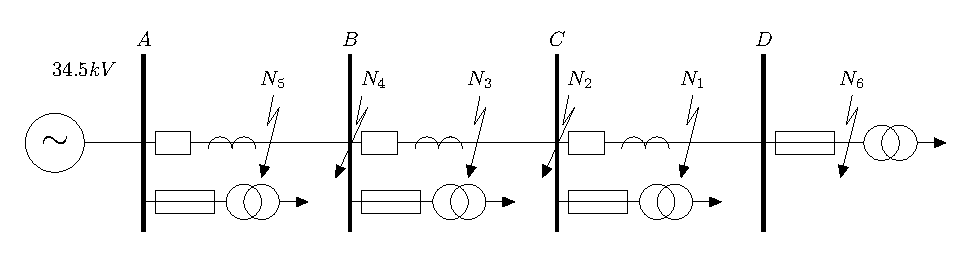
\includegraphics[scale=1]{diagram-draw-tikz/Figure-baitap-baovedongdien-bt2.pdf} 				
				\end{center}
				\vspace{-.5cm}
				\caption{Sơ đồ mạng điện trong bài tập \ref{ex:bt2-bvdongdien} -- bảo vệ dòng điện cực đại với thời gian phụ thuộc} \label{Fig:bt2-bvdongdien}
				\vspace{-.5cm}
			\end{figure}
			
			\subparagraph{Yêu cầu} Xác định các giá trị đặt của bảo vệ dòng điện tại các vị trí $A, B, C$ với đường cong theo tiêu chuẩn của Mỹ có độ dốc $U_2$.
			
			\subparagraph{Bài giải}
				\begin{itemize}
					\item \textbf{Relay C}
						\begin{itemize}
							\item Dòng tải tại thanh cái $C$: $I_{t_C} = \dfrac{S}{\sqrt{3} U} = \dfrac{5 \times 10^6}{\sqrt{3} \times 34.5 \times 10^3} = 83.67 \unit{A}$.
							
							\item Chọn tỉ số $BI$ là $100/5$ và $n_{BI_C} = 20$.
							
							\item Dòng khởi động bảo vệ: $\viet{I}{kđC} = 2 I_{t_C} = 2 \times 83.67 = 167.34 \unit{A}$.
							
							\item Dòng khởi động relay: $\viet{I}{kđRC} = \dfrac{\viet{I}{kđC}}{n_{BI_C}} = \dfrac{167.34}{20} = 8.37 \unit{A}$.
							
							\item Tại điểm $N_6$ dòng ngắt mạch $I_{Nmax} = 350 \unit{A}$ và thời gian cắt của cầu chì $t_{cc} = 3 \unit{s}$ (bảng \ref{Tab:bt2-bvdongdien-dactinh-cauchi}). Suy ra, thời gian cắt của relay $C$ khi có ngắn mạch tại $N_6$:
								\begin{align*}
									t_C = t_{cc} + \Delta t = 3 + 0.3 = 3.3 \unit{s}
								\end{align*}
								
							\item Bội số dòng ngắn mạch so với đặc tính bảo vệ: $m_C = \dfrac{I_{Nmax}}{\viet{I}{kđC}} = \dfrac{350}{167.34} = 2.09$.
							
							\item Phương trình đường cong theo tiêu chuẩn Mỹ với độ dốc $U_2$:
								\begin{align*}
									t_C = \left({0.18 + \dfrac{5.95}{m_C^2 - 1}}\right)TD	\Longleftrightarrow 3.3 = \left({0.18 + \dfrac{5.95}{2.09^2 - 1}}\right)TD \Longleftrightarrow TD = 1.69
								\end{align*}	
							
							\item Chọn $TD = 2$ (làm tròn lên).
							
							\item Tại $N_1$: $I_{Nmax} =743.3 \unit{A}$, suy ra: bội số dòng ngắn mạch $m = \dfrac{I_{Nmax}}{\viet{I}{kđC}} = \dfrac{743.3}{167.34} = 4.44$. Thay vào phương trình đường cong với độ dốc $U_2$:
								\begin{align*}
									t_C = \left({0.18 + \dfrac{5.95}{m^2 - 1}}\right)TD = \left({0.18 + \dfrac{5.95}{4.44^2 - 1}}\right) \times 2 = 1 \unit{s}
								\end{align*}								
						\end{itemize}
						
						\item \textbf{Relay B}
						\begin{itemize}
							\item Dòng tải tại thanh cái $B$: $I_{t_B} = \dfrac{S}{\sqrt{3} U} + I_{t_C}= \dfrac{5 \times 10^6}{\sqrt{3} \times 34.5 \times 10^3} + 83.67 = 167.34 \unit{A}$.
							
							\item Chọn tỉ số $BI$ là $200/5$ và $n_{BI_B} = 40$.
							
							\item Dòng khởi động bảo vệ: $\viet{I}{kđB} = 2 I_{t_B} = 2 \times 167.34 = 334.68 \unit{A}$.
							
							\item Dòng khởi động relay: $\viet{I}{kđRB} = \dfrac{\viet{I}{kđB}}{n_{BI_B}} = \dfrac{334.68}{40} = 8.37 \unit{A}$.
							
							\item Khi ngắn mạch tại $N_1$: dòng ngắn mạch lớn nhất $I_{Nmax} = 743.3 \unit{A}$ thì thời gian cắt của relay $C$ là $t_C = 1 \unit{s}$.
							
							\item Suy ra, thời gian cắt của relay $B$ khi có ngắn mạch tại $N_1$:
								\begin{align*}
									t_B = t_{C} + \Delta t = 1 + 0.3 = 1.3 \unit{s}
								\end{align*}
								
							\item Bội số dòng ngắn mạch so với đặc tính bảo vệ: $m_B = \dfrac{I_{Nmax}}{\viet{I}{kđB}} = \dfrac{743.3}{334.68} = 2.22$.
							
							\item Phương trình đường cong theo tiêu chuẩn Mỹ với độ dốc $U_2$:
								\begin{align*}
									t_B = \left({0.18 + \dfrac{5.95}{m_B^2 - 1}}\right)TD	\Longleftrightarrow 1.3 = \left({0.18 + \dfrac{5.95}{2.22^2 - 1}}\right)TD \Longleftrightarrow TD = 0.77
								\end{align*}
								
							\item Chọn $TD = 1$ (làm tròn lên).
							
							\item Tại $N_3$: $I_{Nmax} =1564.1 \unit{A}$, suy ra: bội số dòng ngắn mạch $m = \dfrac{I_{Nmax}}{\viet{I}{kđB}} = \dfrac{1564.1}{334.68} = 4.67$. Thay vào phương trình đường cong với độ dốc $U_2$:
								\begin{align*}
									t_B = \left({0.18 + \dfrac{5.95}{m^2 - 1}}\right)TD = \left({0.18 + \dfrac{5.95}{4.67^2 - 1}}\right) \times 1  = 0.47 \unit{s}
								\end{align*}								
						\end{itemize}
						
					\item \textbf{Relay A}
						\begin{itemize}
							\item Dòng tải tại thanh cái $B$: $I_{t_A} = \dfrac{S}{\sqrt{3} U} + I_{t_B}= \dfrac{5 \times 10^6}{\sqrt{3} \times 34.5 \times 10^3} + 167.34 = 251.01 \unit{A}$.
							
							\item Chọn tỉ số $BI$ là $300/5$ và $n_{BI_A} = 60$.
							
							\item Dòng khởi động bảo vệ: $\viet{I}{kđB} = 2 I_{t_B} = 2 \times 251.01 = 502.02 \unit{A}$.
							
							\item Dòng khởi động relay: $\viet{I}{kđRA} = \dfrac{\viet{I}{kđA}}{n_{BI_A}} = \dfrac{502.02}{60} = 8.37 \unit{A}$.
							
							\item Khi ngắn mạch tại $N_3$: dòng ngắn mạch lớn nhất $I_{Nmax} = 1564.1 \unit{A}$ thì thời gian cắt của relay $B$ là $t_C = 0.47 \unit{s}$.
							
							\item Suy ra, thời gian cắt của relay $A$ khi có ngắn mạch tại $N_5$:
								\begin{align*}
									t_A = t_{B} + \Delta t = 0.47 + 0.3 = 0.77 \unit{s}
								\end{align*}
								
							\item Bội số dòng ngắn mạch so với đặc tính bảo vệ: $m_A = \dfrac{I_{Nmax}}{\viet{I}{kđA}} = \dfrac{1564.1}{502.02} = 3.12$.
							
							\item Phương trình đường cong theo tiêu chuẩn Mỹ với độ dốc $U_2$:
								\begin{align*}
									t_C = \left({0.18 + \dfrac{5.95}{m_A^2 - 1}}\right)TD	\Longleftrightarrow 0.77 = \left({0.18 + \dfrac{5.95}{3.12^2 - 1}}\right)TD \Longleftrightarrow TD = 0.89
								\end{align*}
							
							\item Chọn $TD = 1$ (làm tròn lên).
							
							\item Tại $N_5$: $I_{Nmax} =3342 \unit{A}$, suy ra: bội số dòng ngắn mạch $m = \dfrac{I_{Nmax}}{\viet{I}{kđA}} = \dfrac{3342}{502.02} = 6.65$. Thay vào phương trình đường cong với độ dốc $U_2$:
								\begin{align*}
									t_A = \left({0.18 + \dfrac{5.95}{m^2 - 1}}\right)TD = \left({0.18 + \dfrac{5.95}{6.65^2 - 1}}\right) \times 1 = 0.32 \unit{s}
								\end{align*}
						\end{itemize}
				\end{itemize}			
	\end{enumerate}

\newpage
\section{Bảo vệ dòng điện có hướng}
\subsection{Nguyên tắc hoạt động}
	\begin{itemize}
		\item Với các mạng cung cấp điện hình vòng và mạch có hai nguồn cung cấp thì bảo vệ dòng cực đại có thời gian làm việc chọn theo từng cấp không thể đảm bảo cắt ngắn mạch một cách chọn lọc.
		
		\item Với các mạng điện trên, người ta dùng bảo vệ dòng điện có hướng. Trong bảo vệ dòng điện có hướng, relay công suất làm nhiệm vụ định hướng công suất.
		
		\item Mã số relay:
			\begin{itemize}
				\item Relay quá dòng có định hướng: $67$.
				
				\item Relay định hướng công suất: $32$.
			\end{itemize}
		
		\item Cấu trúc của bảo vệ dòng điện có hướng: hình \ref{Fig:sodocautruc-bvdongdiencohuong}. Gồm 3 bộ phận chính: bộ phận khởi động -- $RI$, bộ phận định hướng -- $RW$, bộ phận trễ -- $RT$.
			\begin{figure}[!h]
				\begin{center}					
					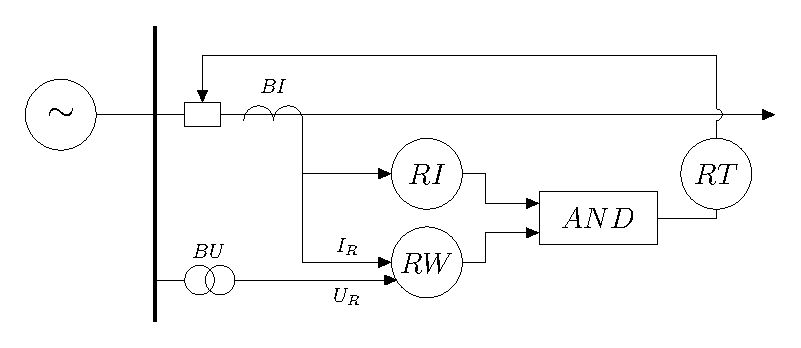
\includegraphics[scale=1]{diagram-draw-tikz/Figure-cautruc-baove-dongdiencohuong.pdf} 
				\end{center}
				\caption{Sơ đồ cấu trúc của bảo vệ dòng điện có hướng} \label{Fig:sodocautruc-bvdongdiencohuong}
			\end{figure}

		\item Bảo vệ dòng điện có hướng tác động khi có dòng ngắn mạch đi từ thanh góp ra đường dây theo cùng chiều của bảo vệ. Ví dụ trên hình \ref{Fig:viduminhhoa-bvdongdiencohuong}, khi ngắn mạch tại $N_1$ thì các bảo vệ $1, 3, 4, 6$ khởi động.
			\begin{figure}[!h]
				\begin{center}					
					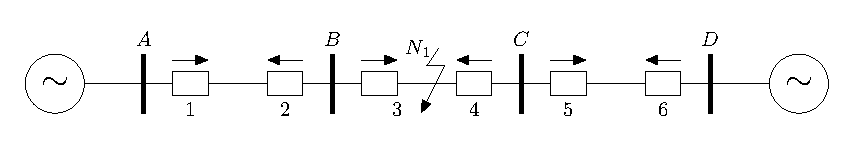
\includegraphics[scale=1]{diagram-draw-tikz/Figure-viduminhhoa-baove-dongdiencohuong.pdf} 
				\end{center}
				\caption{Ví dụ minh họa tác động của bảo vệ dòng điện có hướng} \label{Fig:viduminhhoa-bvdongdiencohuong}
			\end{figure}
	\end{itemize}

\subsection{Phần tử định hướng công suất}	
	\begin{itemize}
		\item Phần tử định hướng công suất có nhiệm vụ định hướng cho bảo vệ, cần có các yêu cầu sau:
			\begin{itemize}
				\item Tác động nhanh.
				
				\item Độ tin cậy cao, muốn vậy thì giá trị công suất và điện áp phải nhỏ đến mức có thể.
				
				\item Loại trừ hiện tượng tự quay khi chỉ có $U$ hoặc $I$.				
			\end{itemize}
			
		\item Phân loại theo nguyên lý làm việc: relay cảm ứng, relay điện động, relay cảm ứng điện động,\ldots
		
		\item Cấu tạo của relay cảm ứng: mạch từ (tạo các cặp cực), trống quay (rotor), lõi thép, tiếp điểm động, tiếp điểm tĩnh, cuộn dòng và cuộn áp (hình \ref{Fig:cautao-relay-dinhhuongcongsuat}).				
		
			\begin{figure}[!h]
				\begin{center}					
					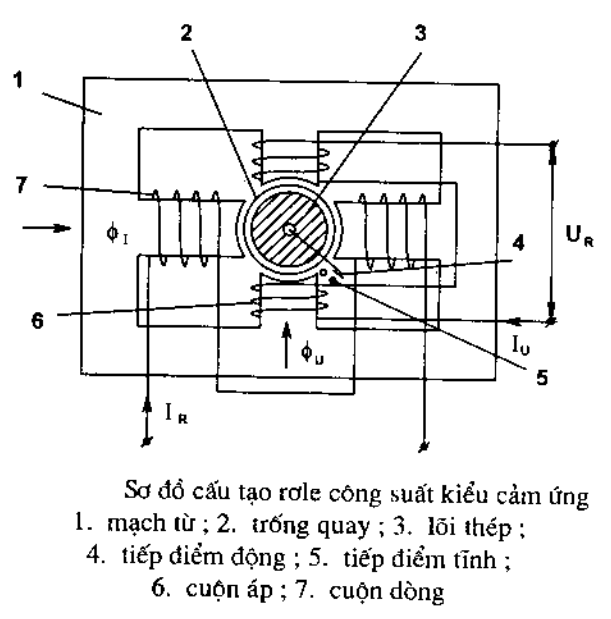
\includegraphics[scale=.5]{images/relay-dinhhuong-cuongsuat.png} 
				\end{center}
				\caption{cấu trúc của relay định hướng công suất kiểu cảm ứng} \label{Fig:cautao-relay-dinhhuongcongsuat}
			\end{figure}
	
		\item Nguyên lý hoạt động của relay định hướng công suất kiểu cảm ứng: khi có dòng điện $I_R$ và điện áp $U_R$ đưa vào các cuộn dây, thì tạo ra từ thông, dưới tác dụng của từ thông tạo ra moment quay. Khi moment quay lớn hơn moment cản thì relay định hướng công suất sẽ tác động.
	\end{itemize}
	
\subsection{Tính toán bảo vệ có hướng}
	\begin{itemize}
		\item Dòng khởi động của bảo vệ cần thỏa hai điều kiện sau: $\viet{I}{kđ} > I_{lvmax}$ và $\viet{I}{kđ} > \viet{I}{pha lành}$.
			\begin{itemize}
				\item Dòng khởi động của bảo vệ: $\viet{I}{kđ} = \dfrac{K_{at} K_{mm}}{K_{tv}} \times I_{lvmax}$.
				
				\item Với ngắn mạch một pha trong mạng điện có trung tính nối đất: $\viet{I}{kđ} = K_{at}\viet{I}{pha lành}$.								
				
				\item Dòng khởi động relay: $\viet{I}{kđR} = \dfrac{K_{at} K_{mm}}{K_{tv} n_{BI}} \times I_{lvmax} = \dfrac{\viet{I}{kđ}}{n_{BI}}$.
				
				\item[$\ast$] Trong đó: $K_{at}$ là hệ số an toàn, $K_{mm}$ là hệ số mở máy động cơ (thường cho $K_{mm} = 2 \div 3$), $K_{tv}$ là hệ số trở về, $n_{BI}$ là tỉ số biến dòng, $I_{lvmax}$ là dòng làm việc cực đại, $\viet{I}{pha lành}$ là dòng điện của pha lành khi xẩy ra ngắn mạch một pha chạm đất ở một pha khác.	
			\end{itemize}				

		\item Độ nhạy của bảo vệ $RI$: $K_{nh} = \dfrac{I_{Nmin}}{\viet{I}{kđ}}$, với $I_{Nmin}$ là dòng ngắn mạch nhỏ nhất trong vùng bảo.
		
		\item Thời gian tác động của bảo vệ: chọn theo quy tắc bậc thang ngược chiều. Ví dụ sơ đồ trên hình \ref{Fig:sodo-baove-dongdiencohuong}.
		
			\begin{figure}[!h]
				\begin{center}					
					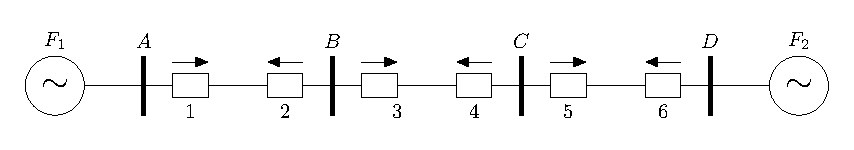
\includegraphics[scale=1]{diagram-draw-tikz/Figure-sodo-baove-dongdiencohuong.pdf} 
				\end{center}
				\caption{cấu trúc của relay định hướng công suất kiểu cảm ứng} \label{Fig:sodo-baove-dongdiencohuong}
			\end{figure}
	
			\begin{itemize}
				\item Thời gian nhóm 1 (tính từ máy phát $F_1$) cần thỏa:
					\begin{list}{+}{}
						\item Gồm các bảo vệ $1, 3, 5$ thì $t_5 < t_3 < t_1$.
						\item Cài đặt thời gian cho nhóm 1: $t_3 = t_5 + \Delta t$ và $t_1 = t_3 + \Delta t$.						
					\end{list}
				
				\item Thời gian nhóm 2 (tính từ máy phát $F_2$) cần thỏa:
					\begin{list}{+}{}
						\item Gồm các bảo vệ $6, 4, 2$ thì $t_2 < t_4 < t_6$.
						\item Cài đặt thời gian cho nhóm 2: $t_4 = t_2 + \Delta t$ và $t_6 = t_4 + \Delta t$.						
					\end{list}
				\item Có nhiều nhánh thì chọn thời gian $t_{max}$ để tính toán cho bảo vệ.
			\end{itemize}
		\item Vị trí cần đặt bộ phận định hướng công suất:
			\begin{itemize}
				\item Không phải bảo vệ nào cũng cần đặt bộ phận định hướng công suất.
				\item  Xét bảo vệ ở hai đầu của một đường dây: bảo vệ nào có thời gian tác động nhỏ hơn thì cần đặt bộ phận định hướng công suất.
				\item Nếu thời gian tác động của bảo vệ ở hai đầu đường dây bằng nhau thì không cần đặt bộ phận định hướng công suất.
			\end{itemize}		
	\end{itemize}
	
\subsection{Một số mạng điện cần áp dụng bộ phận định hướng công suất cho bảo vệ dòng điện}
	\begin{itemize}
		\item Hai đường dây song song với hai nguồn cung cấp.
		
		\item Đường dây có hai nguồn cung cấp từ hai phía.
		
		\item Mạng vòng kín một nguồn cung cấp.
		
		\item Mạng vòng kín có nhiều nguồn cung cấp.
	\end{itemize}
	
\subsection{Đánh giá bảo vệ dòng điện có hướng}
	\begin{itemize}	
		\item \emph{Ưu điểm:}
		\begin{itemize}
			\item Bảo vệ dòng điện có hướng: đơn giản và đảm bảo tác động chọn lọc đối với mạng điện được cung cấp từ hai phía.
		
			\item Sử dụng kết hợp cắt nhanh có hướng với bảo vệ dòng điện có hướng, nhận được bảo vệ với độ nhạy cao, thời gian tác động thỏa mãn yêu cầu.
		
			\item Bảo vệ làm việc chắc chắn.
		\end{itemize}
		
		\item \emph{Nhược điểm:}
			\begin{itemize}
				\item Thời gian tác động khá lớn, nhất là bảo vệ gần nguồn.
				
				\item Có độ nhạy kém trong mạng với phụ tải lớn và bội số dòng ngắn mạch nhỏ.
				
				\item Có vùng chết khi ngắn mạch ba pha.
			\end{itemize}
		
		\item \emph{Phạm vi áp dụng:} dùng làm bảo vệ chính trong các mạng điện lên đến $35 \unit{kV}$ được cung cấp từ hai phía.
	\end{itemize}
%\newpage
\subsection{Bài tập Bảo vệ dòng điện có hướng}
	\begin{enumerate}
		\item \label{ex:bt1-bvdongdiencohuong} Cho mạng điện như hình \ref{Fig:bt1-bvdongdiencohuong}, các số liệu tính toán cho ở bảng \ref{Tab:bt1-baovedongdiencohuong}. Cho $\Delta t = 0.5 \unit{s}$.
			
			\begin{figure}[!h]
				\begin{center}
					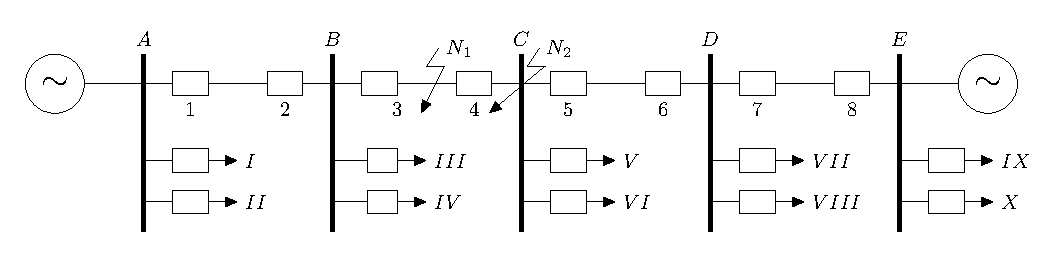
\includegraphics[scale=1]{diagram-draw-tikz/Figure-baitap-baovedongdiencohuong-bt1.pdf}
				\end{center}
				\caption{Sơ đồ mạng điện trong bài tập \ref{ex:bt1-bvdongdiencohuong} -- bảo vệ dòng điện có hướng} \label{Fig:bt1-bvdongdiencohuong}
			\end{figure}
			
			\begin{table}[!h]
				\begin{center}
					\begin{tabular}{|c|c|c|c|c|c|c|c|c|c|c|}\hline 
					\textbf{Phương án} & $t_{I}$ & $t_{II}$ & $t_{III}$ & $t_{IV}$ & $t_{V}$ & $t_{VI}$ & $t_{VII}$ & $t_{VIII}$ & $t_{IX}$ & $t_{X}$ \\ \hline 
					\textbf{1} & 1.5 & 2 & 3.5 & 1.5 & 4 & 2.5 & 3 & 1 & 2 & 1.5 \\ \hline 
					\textbf{2} & 0.5 & 1 & 1.5 & 1.5 & 2 & 2.5 & 3 & 1.5 & 4 & 0.5 \\ \hline 
					\textbf{3} & 1 & 0.5 & 1.5 & 1.5 & 2 & 1 & 1 & 0.5 & 1.5 & 1 \\ \hline 
					\end{tabular} 
				\end{center}
				\caption{Bảng số liệu dùng tính toán cho bài tập \ref{Fig:bt1-bvdongdiencohuong}} \label{Tab:bt1-baovedongdiencohuong}
				\vspace{-.8cm}
			\end{table}
			
			\subparagraph{Yêu cầu}
				\begin{enumerate}[a.]
					\item Chọn thời gian làm việc của bảo vệ dòng điện cực đại có hướng, có đặc tính thời gian độc lập tại các vị trí máy cắt $\pfm{1, 2, 3, 4, 5, 6, 7, 8}$.
					
					\item Cho biết bảo vệ tại vị trí nào cần đặt và không cần đặt bộ phận định hướng công suất $RW$.
					
					\item Giải thích cách làm việc của hệ thống bảo vệ khi có ngắn mạch tại $N_1$ và $N_2$.
				\end{enumerate}
				
			\subparagraph{Bài giải}
				\begin{itemize}
					\item Giả sử hướng công suất ngắn mạch từ thanh góp ra đường dây, chia thành 2 nhóm:
						\begin{itemize}
							\item Nhóm 1: Gồm các bảo vệ $1, 3, 5, 7$.
							
							\item Nhóm 2: Gồm các bảo vệ: $8, 6, 4, 2$.
						\end{itemize}
						
					\item \textbf{Phương án 1}
				\end{itemize}
				
				\begin{enumerate}[\it a.]
				\item \emph{Chọn thời gian làm việc của bảo vệ dòng điện cực đại có hướng}
					\begin{itemize}					
						\item Nhóm 1:
							\begin{itemize}
								\item Relay BV $7$: $t_7 = \max\pfm{t_{IX}, t_{X}} + \Delta t = \max\pfm{2; 1.5} + 0.5 = 2 + 0.5 = 2.5 \unit{s}$.
								
								\item Relay BV $5$: $t_5 = \max\pfm{t_{VII}, t_{VIII}, t_7} + \Delta t = \max\pfm{3; 1; 2.5} + 0.5 = 3 + 0.5 = 3.5 \unit{s}$.
								
								\item Relay BV $3$: $t_3 = \max\pfm{t_{V}, t_{VI}, t_5} + \Delta t = \max\pfm{4; 2.5; 3.5} + 0.5 = 4 + 0.5 = 4.5 \unit{s}$.
								
								\item Relay BV $1$: $t_1 = \max\pfm{t_{III}, t_{IV}, t_3} + \Delta t = \max\pfm{3.5; 1.5; 4.5} + 0.5 = 4.5 + 0.5 = 5 \unit{s}$.			
							\end{itemize}
						
						\item Nhóm 2:
							\begin{itemize}
								\item Relay BV $2$: $t_2 = \max\pfm{t_{I}, t_{II}} + \Delta t = \max\pfm{1.5; 2} + 0.5 = 2 + 0.5 = 2.5 \unit{s}$.
								
								\item Relay BV $4$: $t_4 = \max\pfm{t_{III}, t_{IV}, t_2} + \Delta t = \max\pfm{3.5; 1.5; 2.5} + 0.5 = 3.5 + 0.5 = 4 \unit{s}$.
								
								\item Relay BV $6$: $t_6 = \max\pfm{t_{V}, t_{VI}, t_4} + \Delta t = \max\pfm{4; 2.5; 4} + 0.5 = 4 + 0.5 = 4.5 \unit{s}$.
								
								\item Relay BV $8$: $t_8 = \max\pfm{t_{VII}, t_{VIII}, t_6} + \Delta t = \max\pfm{3; 1; 4.5} + 0.5 = 4.5 + 0.5 = 5 \unit{s}$.
							\end{itemize}
					\end{itemize}
					
					\item \emph{Cho biết bảo vệ tại vị trí nào cần đặt và không cần đặt bộ phận định hướng công suất $RW$}
						\begin{itemize}
							\item Xét cho từng cặp bảo vệ ở 2 đầu đường dây:						
							\begin{itemize}
								\item Giữa thanh cái $A$ và $B$ có: $t_1 = 5 \unit{s} > t_2 = 2.5 \unit{s}$, nên chỉ cần đặt bộ phận định hướng $RW$ tại relay BV $2$.
								
								\item Giữa thanh cái $B$ và $C$ có: $t_3 = 4.5 \unit{s} > t_4 = 4 \unit{s}$, nên chỉ cần đặt bộ phận định hướng $RW$ tại relay BV $4$.
								
								\item Giữa thanh cái $C$ và $D$ có: $t_5 = 3.5 \unit{s} < t_6 = 4.5 \unit{s}$, nên chỉ cần đặt bộ phận định hướng $RW$ tại relay BV $5$.
								
								\item Giữa thanh cái $D$ và $E$ có: $t_7 = 2.5 \unit{s} < t_8 = 5 \unit{s}$, nên chỉ cần đặt bộ phận định hướng $RW$ tại relay BV $7$.
								\end{itemize}
								
							\item Kết luận: hình \ref{Fig:bt1-bvdongdiencohuong-pa1}.
								\begin{itemize}
									\item Cần đặt bộ phận định hướng công suất $RW$ tại các relay BV: $2, 4, 5, 7$.
									
									\item Không cần đặt bộ phận định hướng công suất $RW$ tại các relay BV: $1, 3, 6, 8$.
								\end{itemize}
							
							\begin{figure}[!h]
								\begin{center}
									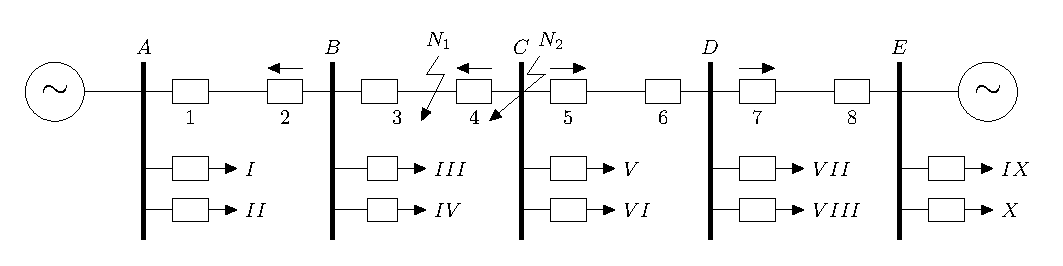
\includegraphics[scale=1]{diagram-draw-tikz/Figure-baitap-baovedongdiencohuong-bt1-pa1.pdf}
							\end{center}
							\caption{Sơ đồ mạng điện trong bài tập \ref{ex:bt1-bvdongdiencohuong} phương án 1 -- bảo vệ dòng điện có hướng} \label{Fig:bt1-bvdongdiencohuong-pa1}
						\end{figure}
						\end{itemize}
						
					\item \emph{Giải thích cách làm việc của hệ thống bảo vệ khi có ngắn mạch tại $N_1$ và $N_2$}
						\begin{itemize}
							\item Khi có ngắn mạch tại $N_1$:
								\begin{itemize}
									\item Các relay BV khởi động khi có sự cố: relay BV $1,3,4,6,8$. Giải thích:
										\begin{list}{+}{}
											\item Các relay không đặt định hướng công suất đều khởi động: relay BV $1, 3, 6, 8$.
											
											\item Theo chiều định hướng công suất (từ thanh góp ra đường dây): chỉ có relay BV 4 là khởi động (relay BV 2 không khởi động).
										\end{list}
										
									\item Các relay BV tác động cắt máy cắt: BV $3, 4$. Giải thích:
										\begin{list}{+}{}			
											\item Thời gian tác động: $t_4 = 4\unit{s} < t_3 = t_6 = 4.5\unit{s} < t_1 = t_8 = 5 \unit{s}$.
											
											\item Do đặc tính chọn lọc: BV $3,4$ sẽ tác động cắt máy cắt.
										\end{list}
								\end{itemize}
								
							\item Khi có ngắn mạch tại $N_2$:
								\begin{itemize}
									\item Các relay BV khởi động khi có sự cố: relay BV $1,3,6,8$. Giải thích:
										\begin{list}{+}{}
											\item Các relay không đặt định hướng công suất đều khởi động: relay BV $1, 3, 6, 8$.
											
											\item Theo chiều định hướng công suất (từ thanh góp ra đường dây): không có relay BV nào khởi động.
										\end{list}
										
									\item Các relay BV tác động cắt máy cắt: BV $3, 6$. Giải thích:
										\begin{list}{+}{}			
											\item Thời gian tác động: $t_3 = t_6 = 4.5\unit{s} < t_1 = t_8 = 5 \unit{s}$.
											
											\item Do đặc tính chọn lọc và thời gian tác động: BV $3,6$ sẽ tác động cắt máy cắt.
										\end{list}
								\end{itemize}
						\end{itemize}
				\end{enumerate}
			
			\begin{itemize}
				\item \textbf{Phương án 2}				
			\end{itemize}

			\begin{enumerate}[\it a.]
			\item \emph{Chọn thời gian làm việc của bảo vệ dòng điện cực đại có hướng}
					\begin{itemize}					
						\item Nhóm 1:
							\begin{itemize}
								\item Relay BV $7$: $t_7 = \max\pfm{t_{IX}, t_{X}} + \Delta t = \max\pfm{4; 0.5} + 0.5 = 4 + 0.5 = 4.5 \unit{s}$.
								
								\item Relay BV $5$: $t_5 = \max\pfm{t_{VII}, t_{VIII}, t_7} + \Delta t = \max\pfm{3; 1.5; 4.5} + 0.5 = 4.5 + 0.5 = 5 \unit{s}$.
								
								\item Relay BV $3$: $t_3 = \max\pfm{t_{V}, t_{VI}, t_5} + \Delta t = \max\pfm{2; 2.5; 5} + 0.5 = 5 + 0.5 = 5.5 \unit{s}$.
								
								\item Relay BV $1$: $t_1 = \max\pfm{t_{III}, t_{IV}, t_3} + \Delta t = \max\pfm{1.5; 1.5; 5.5} + 0.5 = 5.5 + 0.5 = 6 \unit{s}$.			
							\end{itemize}
						
						\item Nhóm 2:
							\begin{itemize}
								\item Relay BV $2$: $t_2 = \max\pfm{t_{I}, t_{II}} + \Delta t = \max\pfm{0.5; 1} + 0.5 = 1 + 0.5 = 1.5 \unit{s}$.
								
								\item Relay BV $4$: $t_4 = \max\pfm{t_{III}, t_{IV}, t_2} + \Delta t = \max\pfm{1.5; 1.5; 1.5} + 0.5 = 1.5 + 0.5 = 2 \unit{s}$.
								
								\item Relay BV $6$: $t_6 = \max\pfm{t_{V}, t_{VI}, t_4} + \Delta t = \max\pfm{2; 2.5; 2} + 0.5 = 2.5 + 0.5 = 3 \unit{s}$.
								
								\item Relay BV $8$: $t_8 = \max\pfm{t_{VII}, t_{VIII}, t_6} + \Delta t = \max\pfm{3; 1.5; 3} + 0.5 = 3 + 0.5 = 3.5 \unit{s}$.
							\end{itemize}
					\end{itemize}
					
					\item \emph{Cho biết bảo vệ tại vị trí nào cần đặt và không cần đặt bộ phận định hướng công suất $RW$}
						\begin{itemize}
							\item Xét cho từng cặp bảo vệ ở 2 đầu đường dây:
							\begin{itemize}
								\item Giữa thanh cái $A$ và $B$ có: $t_1 = 6 \unit{s} > t_2 = 1.5 \unit{s}$, nên chỉ cần đặt bộ phận định hướng $RW$ tại relay BV $2$.
								
								\item Giữa thanh cái $B$ và $C$ có: $t_3 = 5.5 \unit{s} > t_4 = 2 \unit{s}$, nên chỉ cần đặt bộ phận định hướng $RW$ tại relay BV $4$.
								
								\item Giữa thanh cái $C$ và $D$ có: $t_5 = 5 \unit{s} > t_6 = 3 \unit{s}$, nên chỉ cần đặt bộ phận định hướng $RW$ tại relay BV $6$.
								
								\item Giữa thanh cái $D$ và $E$ có: $t_7 = 4.5 \unit{s} > t_8 = 3.5 \unit{s}$, nên chỉ cần đặt bộ phận định hướng $RW$ tại relay BV $8$.								
								\end{itemize}
								
							\item Kết luận: hình \ref{Fig:bt1-bvdongdiencohuong-pa2}.
								\begin{itemize}
									\item Cần đặt bộ phận định hướng công suất $RW$ tại các relay BV: $2, 4, 6, 8$.
									
									\item Không cần đặt bộ phận định hướng công suất $RW$ tại các relay BV: $1, 3, 5, 7$.
								\end{itemize}
							
							\begin{figure}[!h]
								\begin{center}
									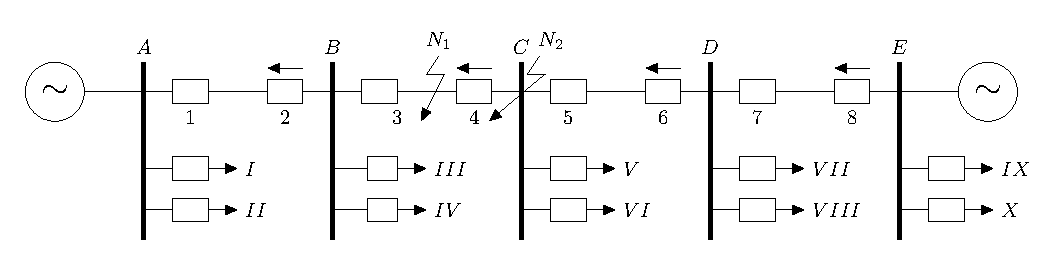
\includegraphics[scale=1]{diagram-draw-tikz/Figure-baitap-baovedongdiencohuong-bt1-pa2.pdf}
							\end{center}
							\caption{Sơ đồ mạng điện trong bài tập \ref{ex:bt1-bvdongdiencohuong} phương án 2 -- bảo vệ dòng điện có hướng} \label{Fig:bt1-bvdongdiencohuong-pa2}
						\end{figure}
						\end{itemize}
						
					\item \emph{Giải thích cách làm việc của hệ thống bảo vệ khi có ngắn mạch tại $N_1$ và $N_2$}
						\begin{itemize}
							\item Khi có ngắn mạch tại $N_1$:
								\begin{itemize}
									\item Các relay BV khởi động khi có sự cố: relay BV $1,3,4,5,6,7,8$. Giải thích:
										\begin{list}{+}{}
											\item Các relay không đặt định hướng công suất đều khởi động: relay BV $1, 3, 5, 7$.
											
											\item Theo chiều định hướng công suất (từ thanh góp ra đường dây): các relay BV $8,6,4$ khởi động (relay BV 2 không khởi động).
										\end{list}
										
									\item Các relay BV tác động cắt máy cắt: BV $3, 4$. Giải thích:
										\begin{list}{+}{}			
											\item Thời gian tác động:
												\begin{align*}												
													t_4 = 2 \unit{s} < t_6 = 3 \unit{s} < t_8 = 3.5 \unit{s} < t_7 = 4.5 \unit{s} < t_5 = 5 \unit{s} < t_3 = 5.5 \unit{s} < t_1 = 6 \unit{s}
											\end{align*}
											
											\item Do đặc tính chọn lọc: BV $3,4$ sẽ tác động cắt máy cắt.
										\end{list}
								\end{itemize}
								
							\item Khi có ngắn mạch tại $N_2$:
								\begin{itemize}
									\item Các relay BV khởi động khi có sự cố: relay BV $1,3,5,6,7,8$. Giải thích:
										\begin{list}{+}{}
											\item Các relay không đặt định hướng công suất đều khởi động: relay BV $1, 3, 5, 7$.
											
											\item Theo chiều định hướng công suất (từ thanh góp ra đường dây): các relay BV $6, 8$ khởi động (relay BV $4, 2$ không khởi động).
										\end{list}
										
									\item Các relay BV tác động cắt máy cắt: BV $3, 6$. Giải thích:
										\begin{list}{+}{}			
											\item Thời gian tác động: $t_6 = 3 \unit{s} < t_5 = 5 \unit{s}$.
											
											\item Mặc dù relay BV 5 gần sự cố $N_2$ hơn relay BV 6 nhưng relay BV 6 có thời gian tác động nhanh hơn nên relay BV 6 tác động trước.
											
											\item Do đặc tính chọn lọc: BV $3,6$ sẽ tác động cắt máy cắt.
										\end{list}
								\end{itemize}
						\end{itemize}
				\end{enumerate}
				
			\begin{itemize}
				\item \textbf{Phương án 3}				
			\end{itemize}

			\begin{enumerate}[\it a.]
			\item \emph{Chọn thời gian làm việc của bảo vệ dòng điện cực đại có hướng}
					\begin{itemize}					
						\item Nhóm 1:
							\begin{itemize}
								\item Relay BV $7$: $t_7 = \max\pfm{t_{IX}, t_{X}} + \Delta t = \max\pfm{1.5; 1} + 0.5 = 1.5 + 0.5 = 2 \unit{s}$.
								
								\item Relay BV $5$: $t_5 = \max\pfm{t_{VII}, t_{VIII}, t_7} + \Delta t = \max\pfm{1; 0.5; 2} + 0.5 = 2 + 0.5 = 2.5 \unit{s}$.
								
								\item Relay BV $3$: $t_3 = \max\pfm{t_{V}, t_{VI}, t_5} + \Delta t = \max\pfm{2; 1; 2.5} + 0.5 = 2.5 + 0.5 = 3 \unit{s}$.
								
								\item Relay BV $1$: $t_1 = \max\pfm{t_{III}, t_{IV}, t_3} + \Delta t = \max\pfm{1.5; 1.5; 3} + 0.5 = 3 + 0.5 = 3.5 \unit{s}$.			
							\end{itemize}
						
						\item Nhóm 2:
							\begin{itemize}
								\item Relay BV $2$: $t_2 = \max\pfm{t_{I}, t_{II}} + \Delta t = \max\pfm{1; 0.5} + 0.5 = 1 + 0.5 = 1.5 \unit{s}$.
								
								\item Relay BV $4$: $t_4 = \max\pfm{t_{III}, t_{IV}, t_2} + \Delta t = \max\pfm{1.5; 1.5; 1.5} + 0.5 = 1.5 + 0.5 = 2 \unit{s}$.
								
								\item Relay BV $6$: $t_6 = \max\pfm{t_{V}, t_{VI}, t_4} + \Delta t = \max\pfm{2; 1; 2} + 0.5 = 2 + 0.5 = 2.5 \unit{s}$.
								
								\item Relay BV $8$: $t_8 = \max\pfm{t_{VII}, t_{VIII}, t_6} + \Delta t = \max\pfm{1; 0.5; 2.5} + 0.5 = 2.5 + 0.5 = 3 \unit{s}$.
							\end{itemize}
					\end{itemize}
					
					\item \emph{Cho biết bảo vệ tại vị trí nào cần đặt và không cần đặt bộ phận định hướng công suất $RW$}
						\begin{itemize}
							\item Xét cho từng cặp bảo vệ ở 2 đầu đường dây:						
							\begin{itemize}
								\item Giữa thanh cái $A$ và $B$ có: $t_1 = 3.5 \unit{s} > t_2 = 1.5 \unit{s}$, nên chỉ cần đặt bộ phận định hướng $RW$ tại relay BV $2$.
								
								\item Giữa thanh cái $B$ và $C$ có: $t_3 = 3 \unit{s} > t_4 = 2 \unit{s}$, nên chỉ cần đặt bộ phận định hướng $RW$ tại relay BV $4$.
								
								\item Giữa thanh cái $C$ và $D$ có: $t_5 = t_6 = 2.5 \unit{s} $, nên không cần thêm bộ phận định hướng công suất $RW$.
								
								\item Giữa thanh cái $D$ và $E$ có: $t_7 = 2 \unit{s} < t_8 = 3 \unit{s}$, nên chỉ cần đặt bộ phận định hướng $RW$ tại relay BV $7$.
								\end{itemize}
								
							\item Kết luận: hình \ref{Fig:bt1-bvdongdiencohuong-pa3}.
								\begin{itemize}
									\item Cần đặt bộ phận định hướng công suất $RW$ tại các relay BV: $2, 4, 7$.
									
									\item Không cần đặt bộ phận định hướng công suất $RW$ tại các relay BV: $1, 3, 5, 6, 8$.
								\end{itemize}
							
							\begin{figure}[!h]
								\begin{center}
									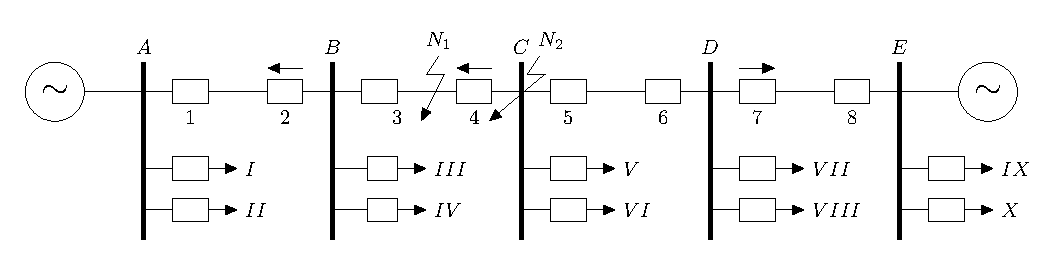
\includegraphics[scale=1]{diagram-draw-tikz/Figure-baitap-baovedongdiencohuong-bt1-pa3.pdf}
							\end{center}
							\caption{Sơ đồ mạng điện trong bài tập \ref{ex:bt1-bvdongdiencohuong} phương án 3 -- bảo vệ dòng điện có hướng} \label{Fig:bt1-bvdongdiencohuong-pa3}
						\end{figure}
						\end{itemize}
						
					\item \emph{Giải thích cách làm việc của hệ thống bảo vệ khi có ngắn mạch tại $N_1$ và $N_2$}
						\begin{itemize}
							\item Khi có ngắn mạch tại $N_1$:
								\begin{itemize}
									\item Các relay BV khởi động khi có sự cố: relay BV $1,3,4,5,6,8$. Giải thích:
										\begin{list}{+}{}
											\item Các relay không đặt định hướng công suất đều khởi động: relay BV $1, 3, 5, 6, 8$.
											
											\item Theo chiều định hướng công suất (từ thanh góp ra đường dây): chỉ relay BV $4$ khởi động (relay BV $2,7$ không khởi động).											
										\end{list}
										
									\item Các relay BV tác động cắt máy cắt: BV $3, 4$. Giải thích:
										\begin{list}{+}{}			
											\item Thời gian tác động: $t_4 = 2\unit{s} < t_5 = t_6 = 2.5\unit{s} < t_3 = t_8 = 3 \unit{s} < t_1 = 3.5 \unit{s}$.
											
											\item Do đặc tính chọn lọc và thời gian tác động: BV $3,4$ sẽ tác động cắt máy cắt.
										\end{list}
								\end{itemize}
								
							\item Khi có ngắn mạch tại $N_2$:
								\begin{itemize}
									\item Các relay BV khởi động khi có sự cố: relay BV $1,3,5,6,8$. Giải thích:
										\begin{list}{+}{}
											\item Các relay không đặt định hướng công suất đều khởi động: relay BV $1, 3, 5, 6, 8$.
											
											\item Theo chiều định hướng công suất (từ thanh góp ra đường dây): không có relay BV nào khởi động.
										\end{list}
										
									\item Các relay BV tác động cắt máy cắt: BV $3, 6$. Giải thích:
										\begin{list}{+}{}			
											\item Thời gian tác động: $t_5 = t_6 = 2.5\unit{s} < t_3 = t_8 = 3 \unit{s} < t_1 = 3.5 \unit{s}$.
											
											\item Do đặc tính chọn lọc: BV $3,6$ sẽ tác động cắt máy cắt.
										\end{list}
								\end{itemize}
						\end{itemize}
				\end{enumerate}
				
			\begin{itemize}			
				\item Tổng hợp kết quả tính toán với 3 phương án trong bài tập \ref{ex:bt1-bvdongdiencohuong}.
					\begin{table}[!h]
						\begin{center}
							\begin{tabular}{|>{\centering\arraybackslash}p{.6cm}|>{\centering\arraybackslash}p{1.5cm}|>{\centering\arraybackslash}p{1.5cm}|>{\centering\arraybackslash}p{1.5cm}|>{\centering\arraybackslash}p{2cm}|>{\centering\arraybackslash}p{2.5cm}|>{\centering\arraybackslash}p{2cm}|>{\centering\arraybackslash}p{2.5cm}|}\hline 
\multirow{3}{1cm}{\textbf{\small P.A}} & \multicolumn{2}{c|}{\textbf{\small Thời gian LV $\mathbf{(s)}$}} & \multirow{3}{1.5cm}{\textbf{\small Vị trí cần đặt $\mathbf{RW}$}} & \multicolumn{2}{c|}{\textbf{\small Ngắn mạch tại $\mathbf{N_1}$}} & \multicolumn{2}{c|}{\textbf{\small Ngắn mạch tại $\mathbf{N_2}$}}  \\ \cline{2-3} \cline{5-8}
								& \multirow{2}{1.6cm}{\textbf{\small Nhóm 1}} & \multirow{2}{1.6cm}{\textbf{\small Nhóm 2}} &  & \multirow{2}{2cm}{\textbf{\small Các BV khởi động}} & \multirow{2}{2.7cm}{\textbf{\small Các BV tác động cắt MC}} & \multirow{2}{2cm}{\textbf{\small Các BV khởi động}} & \multirow{2}{2.7cm}{\textbf{\small Các BV tác động cắt MC}} \\  
								&  &  &  &  &  &  &  \\ \hline 
							\multirow{4}{0.5cm}{\textbf{1}} & $t_1 = 5.0$ & $t_2 = 2.5$ & \multirow{4}{2cm}{2, 4, 5, 7} & \multirow{4}{2cm}{1, 3, 4, 6, 8} & \multirow{4}{1cm}{3, 4} & \multirow{4}{2cm}{1, 3, 6, 8} & \multirow{4}{1cm}{3, 6} \\ \cline{2-3} 
								& $t_3  = 4.5$ & $t_4 = 4.0$ &  &  &  &  &  \\ \cline{2-3} 
								& $t_5  = 3.5$ & $t_6 = 4.5$ &  &  &  &  &  \\ \cline{2-3} 
								& $t_7  = 2.5$ & $t_8 = 5.0$ &  &  &  &  &  \\ \hline
				   			\multirow{4}{0.5cm}{\textbf{2}} & $t_1 = 6.0$ & $t_2 = 1.5$ & \multirow{4}{2cm}{2, 4, 6, 8} & \multirow{4}{2cm}{1, 3, 4, 5, 6, 7, 8} & \multirow{4}{1cm}{3, 4} & \multirow{4}{2cm}{1, 3, 5, 6, 7, 8} & \multirow{4}{1cm}{3, 6} \\ \cline{2-3} 
								& $t_3  = 5.5$ & $t_4 = 2.0$ &  &  &  &  &  \\ \cline{2-3} 
								& $t_5  = 5.0$ & $t_6 = 3.0$ &  &  &  &  &  \\ \cline{2-3} 
								& $t_7  = 4.5$ & $t_8 = 3.5$ &  &  &  &  &  \\ \hline
								\multirow{4}{0.5cm}{\textbf{3}} & $t_1 = 3,5$ & $t_2 = 1.5$ & \multirow{4}{1.2cm}{2, 4, 7} & \multirow{4}{2cm}{1, 3, 4, 5, 6, 8} & \multirow{4}{1cm}{3, 4} & \multirow{4}{2cm}{1, 3, 5, 6, 8} & \multirow{4}{1cm}{3, 6} \\ \cline{2-3} 
								& $t_3  = 3.0$ & $t_4 = 2.0$ &  &  &  &  &  \\ \cline{2-3} 
								& $t_5  = 2.5$ & $t_6 = 2.5$ &  &  &  &  &  \\ \cline{2-3} 
								& $t_7  = 2.0$ & $t_8 = 3.0$ &  &  &  &  &  \\ \hline
							\end{tabular} 
						\end{center}
						\caption{Tổng hợp kết tính toán trong bài tập \ref{ex:bt1-bvdongdiencohuong} -- bảo vệ dòng điện có hướng}
					\end{table}
			\end{itemize}
	\end{enumerate}
	
\newpage
\section{Bảo vệ dòng điện chống chạm đất}
	\subparagraph{Mã số relay}
		\begin{itemize}			
			\item Bảo vệ chống chạm đất: $64$.
			
			\item Bảo vệ quá dòng chống chạm đất: $51G$.
		
			\item Bảo vệ quá dòng chóng chạm đất thời gian trễ: $51N$.
		
			\item Bảo vệ quá dòng cắt nhanh, chống chạm đất: $50N$.			
		
			\item Bảo vệ dòng định hướng, chống chạm đất: $67N$.
		\end{itemize}
		
\subsection{Bảo vệ dòng điện chống chạm đất trong mạng điện có dòng chạm đất lớn}
	Bảo vệ có dòng chạm đất lớn, trung tính nối trực tiếp với đất.
\subsubsection{Bảo vệ dòng cực đại thứ tự không}
	\begin{itemize}
		\item Relay được nối vào bộ lọc dòng thứ tự không.
		\item Thời gian tác động của bảo vệ được chọn theo nguyên tắc bậc thang tăng dần tính từ đầu nhận về phía có máy biến áp có trung tính nối đất.
		
		\item Dòng khởi động của bảo vệ cần thỏa hai điều kiện sau: $\viet{I}{kđ} < 3I_{oNmin}$ và $\viet{I}{kđ} > I_{kcbmax}$.
			\begin{itemize}
				\item Dòng khởi động của bảo vệ: $\viet{I}{kđ} = K_{at} I_{kcbmax}$.
								
				%\item Dòng khởi động relay: $\viet{I}{kđR} = \dfrac{K_{at}}{n_{BI}} \times I_{kcbmax} = \dfrac{\viet{I}{kđ}}{n_{BI}}$.
				
				\item[$\ast$] Trong đó: $K_{at}$ là hệ số an toàn, $I_{kcbmax}$ là dòng không cân bằng cực đại, $I_{oNmin}$ là dòng điện thứ tự không nhỏ nhất.					
			\end{itemize} 
		\item Độ nhạy của bảo vệ: $K_{nh} = \dfrac{3 I_{oNmin}}{\viet{I}{kđ}}$. Yêu cầu: $K_{nh} > 1.5$.
	\end{itemize}
\subsubsection{Bảo vệ dòng cực đại thứ tự không có hướng}
	\begin{itemize}
		\item Bộ phận định hướng công suất xác định dấu hoặc định hướng công suất thứ tự không khi ngắn mạch. Do đó bảo vệ thứ tự không có hướng chỉ tác động khi ngắn mạch xảy ra trên đường dây của bảo vệ.
		
		\item Thời gian tác động của các bảo vệ cùng hướng được chọn theo nguyên tắc bậc thang.		
	\end{itemize}
\subsubsection{Bảo vệ dòng cắt nhanh thứ tự không không có hướng}
	\begin{itemize}
		\item Dùng cho đường dây có dòng $I_o$ chỉ ở một phía khi ngắn mạch chạm đất (trung tính nối đất của máy biến áp nằm về một phía của đường dây), bảo vệ cắt nhanh sẽ tác động tức thời.
		
		\item Dòng khởi động: $\viet{I}{kđ} = 3K_{at} I_{omax}$ với $K_{at}$ là hệ số an toàn và $I_{omax}$ là dòng thứ tự không lớn nhất.
	\end{itemize}

%\subsubsection{Bảo vệ dòng cắt nhanh thứ tự không có hướng}

\subsubsection{Đánh giá và phạm vi sử dụng}
	\begin{itemize}
		\item Bảo vệ thứ tự không được dùng rộng rãi trong mạng điện $110 - 220 \unit{kV}$.
		
		\item \emph{Ưu điểm:} vận hành chính xác, sơ đồ đơn giản và độ tin cậy cao, độ nhạy cao.
		
		\item \emph{Nhược điểm:} bảo vệ phản ứng theo dòng trong chế độ không toàn pha và có thể tác động sai khi đứt dây pha trong mạch thứ cấp của máy biến dòng.
	\end{itemize}
\subsection{Bảo vệ chống chạm đất trong mạng điện có dòng chạm đất nhỏ}
	Bảo vệ có dòng chạm đất nhỏ, trung tính cách điện hoặc nối đất qua cuộn dập hồ quang.
\subsubsection{Những yêu cầu đối với bảo vệ}
	\begin{itemize}
		\item Với mạng điện này, chạm đất không làm tăng cao dòng, không làm biến dạng các đại lượng áp dây, các thiết bị không bị quá tải về dòng, việc cung cấp điện cho các phụ tải không bị ảnh hưởng.
		
		\item Khi chạm đất một điểm, thường bảo vệ chỉ báo tín hiệu, tuy nhiên việc cắt chỗ chạm đất là cần thiết (có thể biến chạm đất một pha thành ngắn mạch giữa các pha; xảy ra hiện tượng tăng áp ở các pha không bị hư hỏng khi có chạm đất, cách điện các pha bị hỏng, tạo nên chạm đất hai pha tại hai điểm khác nhau trong mạng điện).
	\end{itemize}
\subsubsection{Nguyên tắc thực hiện bảo vệ}
	\begin{itemize}
		\item Bảo vệ phản ứng theo dòng thứ tự không.
		
		\item Bảo vệ phản ứng theo dòng dư ổn định đi qua đường dây bị hư hỏng trong trường hợp mạng điện được bù hoàn toàn.
		
		\item Bảo vệ phản ứng theo dòng trong giai đoạn quá độ xuất hiện ở điểm đầu khi xảy ra sự cố.
	\end{itemize}
\end{document}